%! TeX root = main.tex
\documentclass[12pt, a4paper]{article}

% ======================
% Encoding & fonts (XeLaTeX)
% ======================
\usepackage{fontspec} % Handles UTF-8 properly
\setmainfont{Palatino Linotype} % Palatino font
\linespread{1.3}

% ======================
% Geometry & layout
% ======================
\usepackage[margin=2.2cm]{geometry}
\usepackage{ragged2e,setspace} % Alignment & spacing

% ======================
% Graphics & colors
% ======================
\usepackage{graphicx,xcolor}
\usepackage{soul}       % Highlighting text
\usepackage{adjustbox}  % Resize/adjust figures

% ======================
% Figures & tables
% ======================
\usepackage{subcaption} % Subfigures
\usepackage[justification=raggedright,singlelinecheck=false]{caption}
\usepackage{tabularx, multirow, booktabs, makecell} % Tables
\usepackage{float}      % Float positioning
\usepackage{placeins}   % Prevent floats from moving past sections

% ======================
% Math & symbols
% ======================
\usepackage{amsmath, amsfonts, amssymb, latexsym}

% ======================
% Citations & bibliography
% ======================
\usepackage[style=apa, backend=biber]{biblatex} 
\addbibresource{shocks_ineq.bib}

% ======================
% Lists
% ======================
\usepackage[inline]{enumitem}

% ======================
% Footnotes
% ======================
\usepackage[hang,flushmargin]{footmisc}

% ======================
% Hyperlinks
% ======================
\usepackage[colorlinks=true, citecolor=blue, linkcolor=black, urlcolor=blue]{hyperref}

% ======================
% Utilities
% ======================
\usepackage{verbatim, multicol}
\usepackage{dirtytalk} % Proper quotation marks

% ======================
% Custom symbols
% ======================
\newcommand{\sym}[1]{\ifmmode^{#1}\else\(^{#1}\)\fi}
\makeatletter
\def\@fnsymbol#1{\ensuremath{\ifcase#1\or \dagger\or \ddagger\or
   \mathsection\or \mathparagraph\or \|\or **\or \dagger\dagger
   \or \ddagger\ddagger \else\@ctrerr\fi}}
\makeatother

\interfootnotelinepenalty=10000 % Keep large footnotes on one page

% ======================
% Title & authors
% ======================
\title{Shocks and income inequality\thanks{Corresponding author: Oleg Gurshev. Email: o.gurshev@grape.org.pl. Financial support from the Polish National Science Center (grant no. 2021/43/B/HS4/03241) is gratefully acknowledged.}}

\author{
    Oleg Gurshev \\ 
    \small{FAME$\mid$GRAPE} 
    \and 
    Lucas van der Velde \\ 
    \small{FAME$\mid$GRAPE} \\[-0.5em] 
    \small{Warsaw School of Economics}
}
\date{}

% ======================
% Optional: allow slightly looser line-breaking to avoid overfull boxes
% ======================
\sloppy

\begin{document}

\maketitle

\thispagestyle{empty}
% \renewcommand{\thefootnote}{}  % Suppress footnote numbering
% \footnotetext{$\dagger$ Corresponding author. Email: o.gurshev@grape.org.pl.\\Financial support from the Polish National Science Center (grant no. 2021/43/B/HS4/03241) is gratefully acknowledged.}
% \renewcommand{\thefootnote}{\arabic{footnote}} 
% Abstract
\begin{abstract}
\noindent 
% Oleg: changed confidence -> expectations
% Oleg: changed wording in the second sentence and added some additional description to reflect the newly put results
We examine the contribution of supply and demand shocks to income inequality in a panel setting. Leveraging the newly created Global Repository of Income Dynamics, we study the relationship between unanticipated supply and demand shocks and income inequality, distinguishing between domestic and international (US) shocks. Our results show that shocks originating in the United States, on average, increase income dispersion in other developed countries in a procyclical manner: positive demand shocks tend to produce stronger reactions than supply shocks. Decomposing these effects reveals that shocks primarily alter the asymmetry of income changes rather than the overall level of income volatility. We explore different transmission channels: trade, financial and expectations. The trade channel appears particularly relevant for supply shocks. Comparing these external shocks with domestic counterparts, we find that domestic demand shocks exhibit similar dynamics, while domestic supply shocks are associated with declines in income inequality.
\end{abstract}

\bigskip
\hspace*{15pt}\textbf{Keywords:} Inequality; Macroeconomic shocks; Administrative data
 
\hspace*{15pt}\textbf{JEL Classification:} J30, J31, E24, E32
\clearpage


% Done
% Intro - results + contribution (WIP done)
% Abstract - needs 1 sentence (WIP done)

% Todo list before Oct 2025:
% Results - result description (need description of 3 figures + revision of the older text) + possible framing related to the other studies
% Conclusion - need an update summary of the results

% if possible - add BE shocks somewhere (if appropriate)


%--------------------------------------------------------------------------------------
% List of changes - September 2025:
% - Added more recent studies that focus on US shock spillovers to the 2nd paragraph
% - Added more precise framing of the problem in paragraph 2
% - Revised some wording in paragraphs 1 and 3
% - Added additional justification to the use of BQ shocks in paragraph 4
% - Reworked contribution to be in two parts: inequality and shock transmission
% - Extra referencing done in the contribution
% - Revised the description of the results (summary)

% WIP revision - done
\section{Introduction}
% Introductory paragraph
It is now well recognized that the rise in economic inequality across advanced economies over past decades has multiple drivers\footnote{Including, \emph{inter alia}, technological progress \parencite{Bound1995, Acemoglu2002}, demographics \parencite{Karahan2013}, globalization \parencite{feenstra2003global}, labor market structure \parencite{jaumotte2015inequality}, and monetary policy \parencite{coibion2017innocent, furceri2018effects, Amberg2022, andersen2023monetary}.}. However, despite growing attention to the determinants of inequality, there is little systematic empirical evidence on how global shocks to supply and demand shape the entire income distribution, affecting not only overall inequality but also its underlying income dynamics.

% A short intro on demand and supply shocks and why domestic and US shocks can have different effects (with citations) 
At the same time, understanding the origins of international fluctuations continues to be a key area of research. Given the sheer scale and global influence of the United States, its domestic macroeconomic changes are likely to have substantial implications for the global economy and its close economic partners \parencite{Kose2003, Kose2012, kose2017global, kalemli2013global, Fink2015, rey2016, ramey2016macroeconomic, miranda2022global, carrillo2020inquiry, levchenko2020tfp, lakdawala2021international, dees2021global, di2022international, lastauskas2023global}. The impact of these changes is often found to be heterogeneous, with the magnitude of the spillovers on other economies depending critically on their degree of economic integration with the United States. This heterogeneity at the country level strongly suggests that the impact will also be uneven within countries. Yet, surprisingly little is known about the distributional consequences of these external shocks.

% Goal
This paper studies how income distributions react to supply and demand shocks originating in the US and within national economies. To this end, we draw on a rich cross-country database: the Global Repository of Income Dynamics (GRID) by \textcite{guvenen2022global}. This database contains comparable moments of income distributions of unparalleled quality derived from administrative data. Our study analyzes data from countries that participated in the first phase of GRID and meet the minimum data requirements needed for the estimation of shocks: Canada, Denmark, France, Germany, Italy, Mexico, Norway, Spain, and Sweden.

% Methodology
Our analysis proceeds as follows. First, we estimate supply and demand shocks using long-run restrictions\footnote{See characterization of popular identification strategies in \textcite{ramey2016macroeconomic}.} as proposed by  \textcite{blanchard1989dynamic}\footnote{This seminal paper has recently been revisited by \textcite{Binet2015, Herwartz2018, Keating2013}.}. We adopt this approach because its data requirements are minimal, making it particularly suitable for our broad international setting. Specifically, this method imposes restrictions based on economic theory, where supply shocks are assumed to have permanent effects on output, while demand shocks have only temporary effects. The second step involves recovering the reaction of income dispersion to US and country-specific (domestic) shocks using impulse response functions (IRFs) estimated directly from local projections \parencite{jorda2005estimation, jorda2024local}. In this step, we also study the reaction of the income distribution, measured by the standard deviation and the Kelley skewness of the residual first-year log income changes, to these shocks. Finally, we study the three potential transmission channels that are frequently identified in the literature: trade linkages \parencite{corsetti2011multilateral}, financial market integration \parencite{faccini2016international}, and expectations \parencite{klein2021real} using state-dependent local projections in the style of \textcite{auerbach2013output}.

% Result description - WIP
Our findings indicate that supply and demand shocks originating in the United States tend to raise income dispersion abroad. We also confirm that these changes are largely procyclical. Decomposing these dynamics reveals that shocks primarily alter the asymmetry of income changes rather than the overall level of income volatility. While all shocks make the income distribution more positively skewed, the effect on volatility reveals a critical distinction: US supply shocks increase volatility, whereas domestic supply shocks act as a stabilizing force by significantly decreasing it. When considering transmission channels, the distinction between demand and supply shocks is relevant. Demand shocks increase inequality regardless of the level of exposure. By contrast, supply shocks produce more heterogeneous responses.


%The difference in responses is consistent with models of= international trade, where firms participating in international markets are more productive and offer goods of a higher quality. Demand shocks in the US are transmitted to higher wages among the most productive firm abroad, i.e. an export supply channel. We find evidence in favor of this by using responses to US shocks together with trade exposure interaction%.

% Contribution - WIP
This paper makes two main contributions. First, our findings complement the recent body of studies that investigate the dynamic causal link between macroeconomic shocks and the Gini such as \textcite{coibion2017innocent, Davtyan2017, furceri2018effects} by providing novel evidence using a wide variety of broadly defined shocks. Specifically, our analysis goes beyond documenting the impact of shocks on the Gini coefficient, as we also examine their possible effects on the distributional measures using one-year residual log income changes: standard deviation and Kelley skewness, revealing new patterns that have so far received little attention in prior research. Second, we report new evidence related to the transmission of US supply and demand shocks abroad via trade, financial, and expectations channels. Here, our findings complements the growing literature that studies spillover effects and transmission of various shocks originating within the US: \textcite{akinci2013global, bowman2015us, fernandez2017world, schmitt2018important, di2022international, azad2022spillovers, lastauskas2023global, LASTAUSKAS2024101956}. We document the critical importance of all three channels when it comes to US supply shocks. Countries with strong export links to the US tend to experience a significant and lasting rise in inequality. In contrast, countries with high financial exposure experience only a brief increase in inequality immediately following the shock, while those with weaker financial exposure see a gradual rise even after the three-year horizon. Finally, lower domestic business confidence corresponds to a stronger inequality response.

%The comparison between domestic and international shocks reveals fundamental differences. First, domestic shocks generate weaker, and often not statistically significant, responses. Second, domestic supply shocks are associated with a decline in inequality.

The paper is structured as follows. Section 2 describes data and methodology. Section 3 reports the results. Section 4 concludes.

%-----------------------------------------------------------------------------------
% List of changes - September 2025:
% - Changed section and subsection names to better reflect content
% - Moved Tables from Appendix to main text
% - Added necessary text descriptions
% - Added VAR algebra
% - Revised Table 1 to include Kelly and Std

% WIP revision - done
\section{Methodology}

\subsection{Inequality measures and shocks} 
The Global Repository of Income Dynamics (GRID) provides measures of inequality from administrative records across several countries. This source has several advantages. First and foremost, income is less subject to reporting errors, and there is an adequate representation of earners at the top of the income distribution, neither of which is not guaranteed in other databases. Second, estimates are based on larger samples, quite often the entire working population. Finally, GRID also provides better coverage than similar open source databases (OECD, Luxembourg Income Study), as time series are uninterrupted. However, the database has some limitations, namely: i) income refers to labor income at the individual level, ii) since it is based on tax records, envelope payments are not included. As our sample contains mostly developed countries, the bias introduced might not be significant.

All income inequality measures are computed only among individuals between ages 25-55, who are expected to be active in the labor market. To ensure that individuals are attached to the labor markets, the sample used in GRID is further restricted to those perceiving yearly earnings above a minimum threshold (one fourth of the minimum wage). All measures are based on gross earnings\footnote{Each country has it's own specific approach to measuring gross earnings. However, the resulting measures are comparable as they include all forms of compensation subject to taxation and social security contributions (i.e., base salary, overtime compensation, performance and seasonal bonuses, paid vacations, paid sick leaves, and severance payments).} deflated to 2018 price levels. Table \ref{table:a5} presents descriptive statistics (means) for the Gini coefficient together with distributional measures of residual one-year log income changes (standard deviation and Kelley skewness) as collected from GRID.

We recover supply and demand shocks using the long-run restrictions approach pioneered by \textcite{blanchard1989dynamic}. The identification of shocks begins with a reduced-form VAR of order $p$:
\begin{equation} \label{eq:var_reduced}
X_t = \sum_{i=1}^{p} A_i X_{t-i} + e_t
\end{equation}
where $X_t = [\Delta y_t, u_t]'$ is the vector of endogenous variables (growth rate of real output and the unemployment rate), $A_i$ are coefficient matrices, and $e_t$ is a vector of serially uncorrelated reduced-form residuals with covariance matrix $\Omega$.

These reduced-form residuals are linear combinations of the underlying structural shocks, $\epsilon_t = [\epsilon^s_t, \epsilon^d_t]'$, which represent supply and demand shocks, respectively. The relationship is given by:
\begin{equation} \label{eq:shocks_relation}
e_t = S\epsilon_t
\end{equation}
where we assume the structural shocks are orthonormal, i.e., $E[\epsilon_t \epsilon_t'] = I$. To identify the matrix $S$, we consider the moving-average representation of the VAR, $X_t = C(L)e_t = C(L)S\epsilon_t$. The long-run impact of the structural shocks on the variables is given by the matrix $C(1)S$.

The key identifying assumption is that demand shocks ($\epsilon^d_t$) have no long-run effect on the level of output. This economic restriction implies that the cumulative effect of a demand shock on the output growth rate, $\Delta y_t$, must sum to zero. This forces the $(1,2)$ element of the long-run multiplier matrix to be zero, making the matrix lower triangular. This constraint, combined with the condition from the covariance matrix ($SS' = \Omega$), provides the necessary restrictions to uniquely identify the structural shocks.

% Table: panel data coverage (revised variant)
\begin{table}[H]
\captionsetup{justification=raggedright, singlelinecheck=false}
\centering
\caption{Availability of GRID data.}
\small 
\setlength{\tabcolsep}{5pt} 
\renewcommand{\arraystretch}{0.95}
\begin{tabular}{l c c c c}
\toprule
Country & Scope & Gini & Std & Kelley skewness \\
\midrule
Canada   & 1990--2019 & 0.41 (0.01) & 0.53 & 0.02\\
Denmark  & 1990--2016 & 0.28 (0.01) & 0.42 & 0.03\\
France   & 1991--2016 & 0.34 (0.00) & 0.47 & -0.03\\
Germany  & 2001--2016 & 0.40 (0.01) & 0.40 & 0.18\\
Italy    & 1990--2016 & 0.36 (0.02) & 0.48 & 0.03\\
Mexico   & 2005--2019 & 0.56 (0.00) & 0.65 & -0.01\\
Norway   & 1993--2017 & 0.33 (0.01) & 0.59 & -0.01\\
Spain    & 2005--2018 & 0.40 (0.01) & 0.50 & 0.02\\
Sweden   & 1990--2016 & 0.30 (0.01) & 0.49 & 0.04\\
\bottomrule
\end{tabular}

\vspace{0.1cm}
\parbox{0.9\linewidth}{\raggedright\footnotesize Note: own summary. Scope refers to the availability of Gini data. The panel is unbalanced, with a total of $N=217$ country-year observations for the Gini coefficient. Gini is reported as mean (standard deviation). Kelley skewness and standard deviation are from residual one-year log income changes. Their effective coverage is one year shorter at both the start and end of the sample compared to the Gini series. All data are annual.}
\label{table:a5}
\end{table}



Following  this framework, we estimate a bivariate VAR for each country using quarterly rates of unemployment and real output growth\footnote{Lag length is selected using AIC separately for each country: one lag (Canada, Italy, Mexico, Norway), two lags (Denmark, France, Germany, Spain Sweden, USA). Impulse response functions for each country (demand and supply shocks) are available in Figures \ref{fig:var_impulses_demand} and \ref{fig:var_impulses_supply} (Appendix). While demand shocks are temporary, they decay at a slow rate. In some countries, the responses are different from zero even 20 quarters after the initial shock (see Figure \ref{fig:var_impulses_demand} in Appendix).}. We collect the necessary data from the Federal Bank of St. Louis (FRED) and the OECD databases.\footnote{Even if data requirements are minimal, they are not satisfied by every country. Argentina and Brazil lack data on unemployment rates for the early years of the sample. Therefore, we excluded these countries from further analysis.}. All series were de-meaned prior to VAR input. Detailed description of the data used for the estimation of the bivariate models is available in Table \ref{table:a1} (Appendix). Tables \ref{table:a2} and \ref{table:a3} display the correlation of quarterly supply and demand shocks across countries. Shocks generally feature low degree of correlation across countries except the two pairs (DEU-ESP, DEU-FRA). Finally, given that GRID data are available at the yearly level, we annualize and standardize (mean-center and scale to unit variance) the obtained shocks before using them in panel estimation. This transformation ensures comparability across countries, prevents scale effects from biasing the estimates, and facilitates interpretation of the impulse responses in standard deviation units.

% Table A2 supply shock
\begin{table}[H]
\captionsetup{justification=raggedright,
singlelinecheck=false
}
    \centering
    \caption{Pairwise correlations: supply shock.}  
    \begin{tabular}{l ccc ccc ccc c}
    \toprule
 & CAN & DKK & DEU & ESP & FRA & ITA & MEX & NOR & SWE & USA \\ 
  \hline
  CAN & 1 &  &  &  &  &  &  &  &  &  \\ 
  DKK & -0.08 & 1 &  &  &  &  &  &  &  &  \\ 
  DEU & -0.24 & 0.14 & 1 &  &  &  &  &  &  &  \\ 
  ESP & -0.16 & 0.05 & 0.38 & 1 &  &  &  &  &  &  \\ 
  FRA & 0.07 & 0.08 & -0.25 & -0.22 & 1 &  &  &  &  &  \\ 
  ITA & -0.14 & 0.01 & 0.1 & -0.06 & 0.17 & 1 &  &  &  &  \\ 
  MEX & -0.19 & -0.13 & 0.4 & 0.2 & -0.08 & 0.15 & 1 &  &  &  \\ 
  NOR & 0.14 & 0.12 & -0.04 & 0 & -0.02 & 0.05 & 0.02 & 1 &  &  \\ 
  SWE & -0.04 & 0.14 & 0.31 & 0.25 & -0.01 & 0.1 & 0.02 & 0.13 & 1 &  \\ 
  USA & 0.02 & 0.17 & 0.09 & 0.22 & -0.08 & 0.07 & 0.18 & 0.03 & 0.12 & 1 \\ 
  \bottomrule
    \end{tabular}
    \begin{minipage}{\textwidth}
    \vspace{0.1cm} 
    \footnotesize Note: own summary, shocks are obtained using long-run restrictions. The period under analysis is 1990:Q2-2019:Q3 for all countries except Germany (1991:Q2-2019:Q3).
    \end{minipage}
    \label{table:a2}
\end{table}

%-----------------------------------------------------------------------------

% Table A3 demand shock
\begin{table}[H]
\captionsetup{justification=raggedright,
singlelinecheck=false
}
    \centering
    \caption{Pairwise correlations: demand shock.}
    \begin{tabular}{l ccc ccc ccc c}
    \toprule
& CAN & DKK & DEU & ESP & FRA & ITA & MEX & NOR & SWE & USA \\ 
  \hline
  CAN & 1 &  &  &  &  &  &  &  &  &  \\ 
  DKK & 0.2 & 1 &  &  &  &  &  &  &  &  \\ 
  DEU & 0.19 & 0.05 & 1 &  &  &  &  &  &  &  \\ 
  ESP & 0.12 & -0.03 & 0.1 & 1 &  &  &  &  &  &  \\ 
  FRA & 0.24 & 0.17 & 0.36 & -0.01 & 1 &  &  &  &  &  \\ 
  ITA & 0.14 & 0.2 & 0.14 & -0.07 & 0.28 & 1 &  &  &  &  \\ 
  MEX & 0.22 & 0.17 & 0.12 & 0.15 & 0.12 & 0.17 & 1 &  &  &  \\ 
  NOR & 0.13 & 0.23 & -0.11 & -0.02 & 0.13 & 0.14 & 0.1 & 1 &  &  \\ 
  SWE & 0.23 & 0.15 & 0.15 & -0.03 & 0.2 & 0.17 & 0.07 & 0.11 & 1 &  \\ 
  USA & 0.16 & 0.23 & 0.16 & -0.07 & 0.12 & 0.25 & 0.16 & 0.16 & 0.05 & 1 \\ 
    \bottomrule
    \end{tabular}
    \begin{minipage}{\textwidth}
    \vspace{0.1cm}
    \footnotesize Note: own summary, shocks are obtained using long-run restrictions. The period under analysis is 1990:Q2-2019:Q3 for all countries except Germany (1991:Q2-2019:Q3).
    \end{minipage}
    \label{table:a3}
\end{table}


\subsection{Local projections} 
To study the impact of supply and demand shocks on (the level of) inequality, we compute cumulative IRFs directly from local projections. Specifically, we estimate the following regression at the country level:
\begin{equation}
    y_{c,t+h}-y_{c,t-1} =  \beta^h z_{c,t} + \gamma^h_c + \gamma^h_t + \pi^h X_{c,t} + e^h_{c, t+h}
\label{eq:1}
\end{equation}
\noindent where $y_{c,t+h}$ is the log of Gini for country $c$ measured at time $t+h$, $z_{c,t}$ is the exogenous shock, and $\beta^h$ are the estimated responses for $h = 0,..,3$ periods after the shock. The remaining elements identify country fixed effects ($\gamma^h_c$). The next term  ($\gamma^h_t$) addresses potential period differences. When analyzing domestic shocks, $\gamma^h_t$ represent time fixed effects. When shocks originate in the US (and are common to all countries), $\gamma^h_t$ represents NBER-identified recessions in the US (level and two lag values).

Our baseline set of controls ($X_{c,t}$) includes two lags of: changes in inequality ($\Delta y_{c,t-i}$, for $i =1,2$) and exogenous shock used ($z_{c,t-i}$, for $i =1,2$), i.e. supply or demand. As a robustness check, we expand the set of control variables to include two lags of: i) share of exports to the US to total exports (trade exposure), ii) share of US bank claims to GDP (financial exposure), iii) changes in \textit{de facto} economic openness (proxied by the \textit{de facto} component of the KOF index), iv) expectations (proxied by the OECD's business confidence index), and v) changes in domestic labor market policies (proxied by the Economic Freedom of the World's indicator of labor market regulation), see Table \ref{table:a4} for details (Appendix).

To examine the three potential transmission channels of supply and demand shocks originating in the US we apply the state-dependent local projection in the style of \textcite{auerbach2013output}. Namely, we estimate the following regression:
\begin{equation}
    y_{c,t+h}-y_{c,t-1} = \beta^h z^{US}_{t} + \gamma^h (z^{US}_{t} \times s_{c,t-1}) + \pi^h X_{c,t} + \gamma^h_c + e^h_{c, t+h}
\label{eq:2}
\end{equation}
where $s_{c,t-1}$ represents the state variable: i) percentage of exports to US in all exports of country $c$ (trade channel), ii) bilateral US bank claims as a proportion of GDP in country $c$ (financial channel), and iii) business confidence in country $c$ (expectations channel). $X_{c,t}$ includes two lags of: changes in inequality, exogenous shock being used, interaction term, and NBER-identified recessions. The state-dependent cumulative impulse response is the linear combination $\beta^h + \gamma^h \times s_{c,t-1}$.

Finally, all estimations use Driscoll-Kraay standard errors in reporting confidence bands. These standard errors accommodate different forms of autocorrelation and heteroskedasticity.

%-------------------------------------------------------------------------------------
% List of changes - September 2025:
% - Split into two subsections
% - Added results for asymetric impact for US shocks
% - Moved subsample figure from Appendix to main text
% - Added additional results for Kelly and Std

\section{Results}
We report our results as follows. First, we estimate the baseline responses of the Gini coefficient computed for the entire working-age population to unanticipated, one-standard-deviation change in US and domestic shocks. Next, we extend our baseline analysis to two measures of the income distribution. Namely, we replace the Gini coefficient with: i) the standard deviation of these changes, which captures the overall income volatility, and ii) the Kelley skewness of residual one-year log income changes, which measures the asymmetry of income risk. Second, we present the results for the transmission channels of US shocks. Specifically, we capture the state-dependency by including a linear interaction term with the three measures representing trade, financial, and expectations channels.

%Finally, we check robustness of our baseline estimates by including additional controls related to alternative drivers of inequality.

%Finally, we report results using two subpopulations: men and women. 
\subsection{Inequality}
% US supply and demand shocks
The upper row of Figure \ref{fig:demand_supply_base} displays the responses of the log of Gini to demand and supply shocks originating in the US. US demand shock leads to a significant and long-lasting increase (up to 40 basis points) in income inequality. US supply shocks produce much smaller increases in income inequality (up to 25 basis points). Domestic shocks, whether demand or supply, produce IRF in the vicinity of 5 basis points, as shown in the bottom row of Figure  \ref{fig:demand_supply_base}. The direction is less clear than in the case of US shocks. Domestic demand shocks produce an initial hike that quickly vanishes, whereas domestic supply shocks tend to decrease inequality at longer horizons. Overall, domestic demand shocks generate an increase in inequality, though responses remain lower than those to US shocks. Moreover, estimates from the intermediate specification suggest that responses are driven (partly) by sample composition. 

% Figure 2 + 3 description

% Figure 4 - procyclical

% Baseline result
\begin{figure}[H]
    \centering    
    \caption{Cumulative impulse responses to demand and supply shocks: Gini, baseline.}  
    \label{fig:demand_supply_base}
    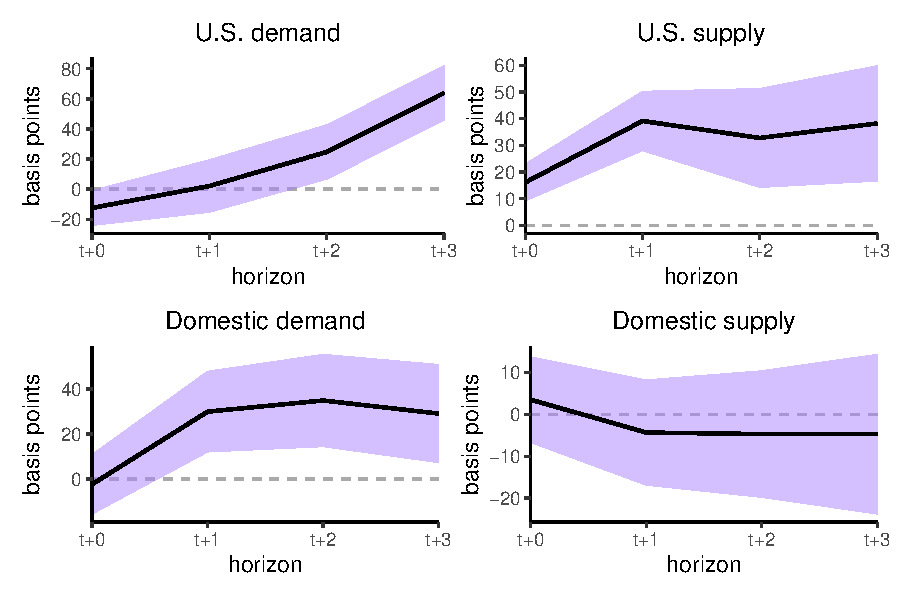
\includegraphics[width=0.75\textwidth]{Figures/baseline_demand_supply_LP_extended.pdf}
    \centering \caption*{Note: shaded areas represent 68\% Driscoll-Kraay confidence bands. Detailed output of our baseline result is available in Table \ref{tab:a7_baseline_reg_output} (Appendix).}
\end{figure}

We conduct a number of robustness exercises. First, we evaluate the evolution of responses beyond the initial estimation horizon of three years, see Figure \ref{fig:irf_longer} (Appendix), given that the panels are short, estimates from these longer horizon are less reliable, which is reflected in the broader confidence bands. To the extent that conclusions are possible, the response to foreign demand shocks decreases over time, whereas foreign supply shocks produce more persistent responses. Further, we check whether the inclusion of additional drivers of the Gini coefficient affects the estimated responses. The new variables include labor market regulations, and the \textit{de facto} component of the KOF globalization index. The resulting IRFs are portrayed in Figure \ref{fig:demand_supply_robust} (Appendix). The patterns described for US demand shocks are robust to the inclusion of new variables. The trajectory of responses to supply shocks is also identical, but shifted downwards. Table \ref{table:a8} presents the estimated coefficients. Since the additional controls are not available each year, we also include  an intermediate specification, which restricts the sample, but does not include any of the additional control variables.

% IRFs for Std
\begin{figure}[H]
    \centering    
    \caption{Cumulative impulse responses to demand and supply shocks: standard deviation, baseline.}  
    \label{fig:std_base}
    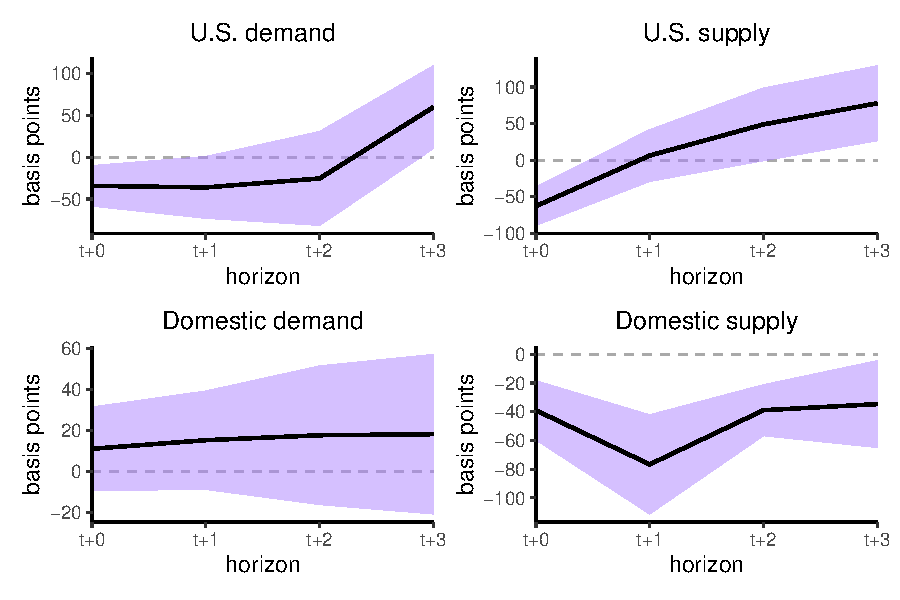
\includegraphics[width=0.75\textwidth]{Figures/std_demand_supply_LP.pdf}
    \centering \caption*{Note: shaded areas represent 68\% Driscoll-Kraay confidence bands.}
\end{figure}

% IRFs for Kelley
\begin{figure}[H]
    \centering    
    \caption{Cumulative impulse responses to demand and supply shocks: Kelley skewness, baseline.}  
    \label{fig:kelley_base}
    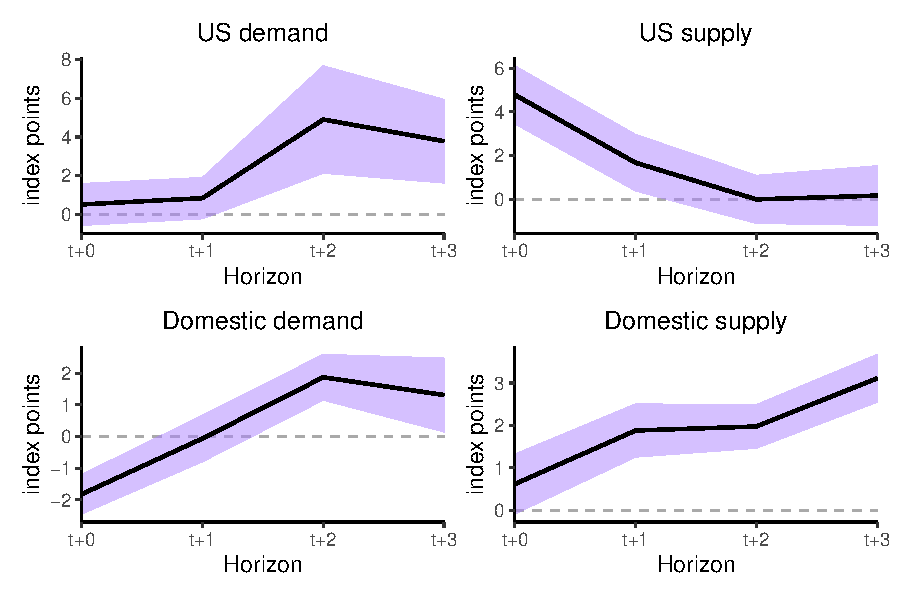
\includegraphics[width=0.75\textwidth]{Figures/kelley_demand_supply_LP.pdf}
    \centering \caption*{Note: shaded areas represent 68\% Driscoll-Kraay confidence bands.}
\end{figure}

% Asymetric shocks
\begin{figure}[H]
    \centering
    \caption{Cumulative state-dependent impulse responses to positive and negative US demand and supply shocks: Gini.}
    \label{fig:demand_supply_asym}
    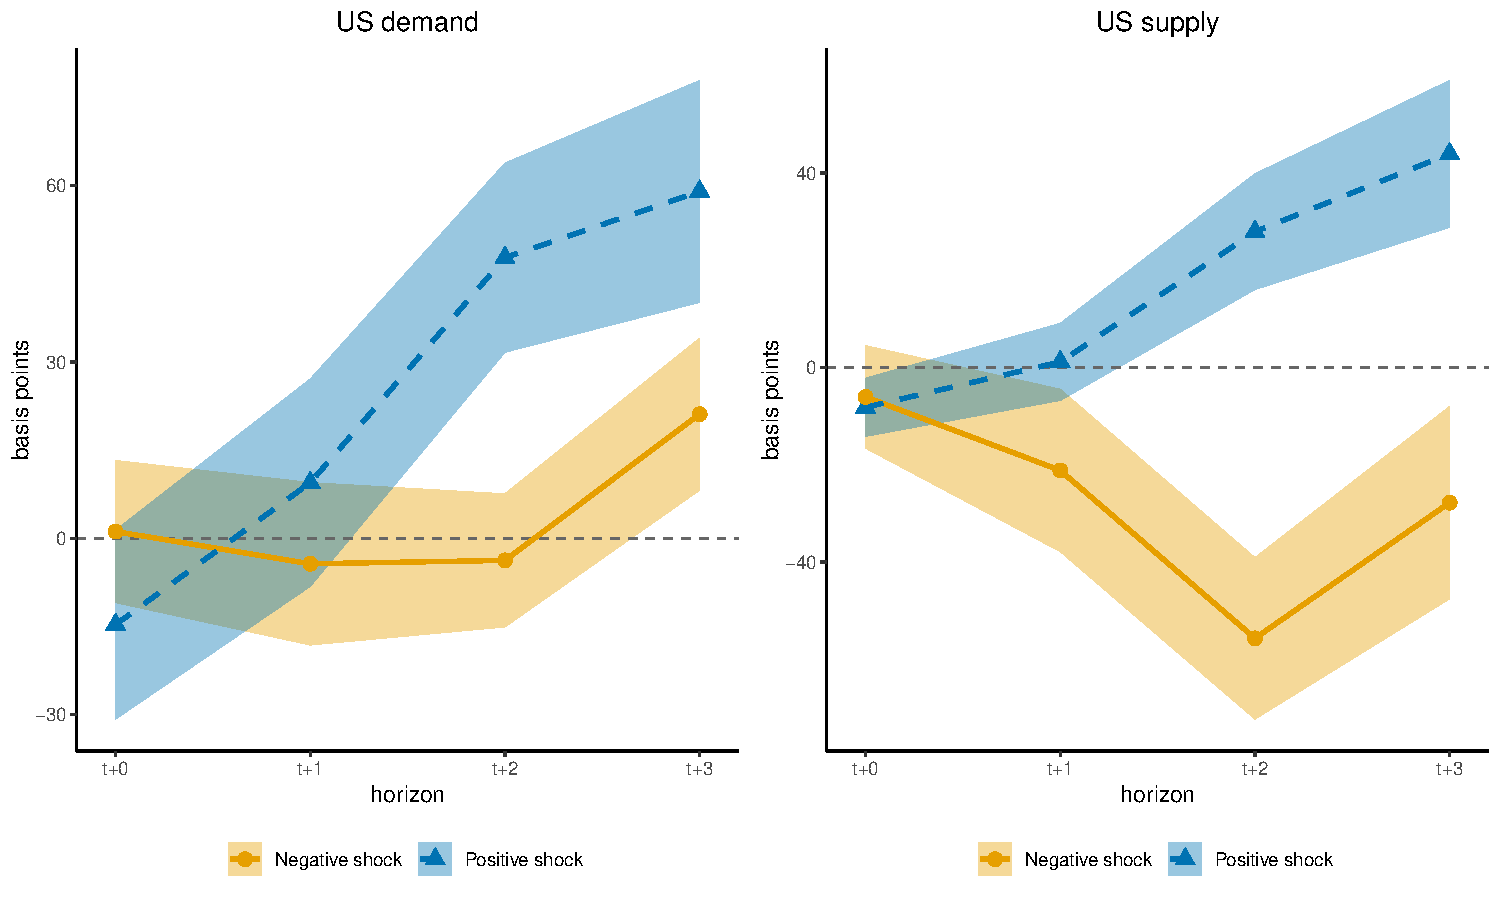
\includegraphics[width=0.80\textwidth]{Figures/asymmetric_IRFs.pdf}
    \centering \caption*{Note: shaded areas represent 68\% Driscoll-Kraay confidence bands.}
\end{figure}

%Estimations are noisier, though, and any conclusion should be taken with some salt.      %We interpret the behavior of the demand shock by the existing inter-market dependencies across our sample, where changes in US demand have a strong impact abroad. As employment is linked with income and current consumption, we think US consumption of foreign goods and services is the main driver behind these responses. This finding is also in line with the existing evidence on economic co-movement between booms and busts occurring in the US vis-a-vis the world \parencite{Kose2003, Kose2012, Fink2015}. 

\subsection{Channels}
In Figure \ref{fig:demand_supply_channels_ag}, we study the three potential transmission channels: trade linkages \parencite{corsetti2011multilateral}, financial markets integration \parencite{faccini2016international}, and expectations \parencite{klein2021real}. None of these channels explains variation in responses to demand shocks. By contrast, supply shocks produce heterogeneous responses based on exposure. When countries have strong export links a US supply shock leads to a large and persistent increase in inequality. Second, countries with strong financial links observe a short-lived increase in inequality during the first period after the shock, whereas countries with weaker links observe a gradual increase in inequality during the entire estimation horizon. Lastly, lower business confidence in home country is associated with a more pronounced inequality response. As an extension of our state-dependent results, we perform a data-driven subsample split using country-level median values of channel measure and estimate our baseline specification (see Figure \ref{fig:demand_supply_channels}). When splitting the countries, demand shocks appear more differentiated by trade level, countries above the median in the initial year have a stronger reaction. 

% Can the result be framed in relation to the other studies?

%splitting the panel between countries that are more (less) exposed to US shocks. In the case of trade, we split the samples based on the percentage of exports to the US as a percentage of all exports\footnote{Canada, Germany, Italy, Mexico,
%Sweden belong to the group of more exposed countries; Denmark, France, Norway and Spain are the least exposed.}. In the case of financial linkages, we split the sample based on  US bank claims in a given country as a percentage of its GDP \footnote{Canada, Denmark, France, Germany, and Mexico belong to the group of more exposed countries;  Italy, Norway,
%Spain, and Sweden are the least exposed.}. 

%The results, plotted in Figure     \ref{fig:demand_supply_channels}, suggest that the trade channel is particularly relevant. More exposed countries react more strongly to both demand and supply shocks in the US. The reaction to demand shocks follows expectations from recent trade literature \parencite{furusawa2019international,adao2022imports}. An increase US demand for foreign goods leads to a reallocation of production towards exporting firms in foreign economies. As these firms tend to pay better, and have a more productive workforce, these changes favor higher earners. The scale of US demand shocks is large due to its sheer economic size \parencite{kose2017global}. Notice that among countries with lower exposure the IRF to US demand shocks are weaker and of an opposite signs. Only as of the third period we observe a reversal of signs, which suggest that the export-led channel might be at work with some lags. In the case of supply shocks, the response is also stronger among countries that have closer ties to the US. As in the previous case, inequality increases. This can reflect an import channel, where imports from the US displace domestic workers in less competitive firms. 

%The second split distinguishes between countries based on their exposure to US claims. Our initial expectation is that more exposed countries would present a stronger reaction, as a negative shocks could pull investments away from foreign countries. Yet, estimated IRF's present similar trajectories, and their confidence intervals present substantial overlap. 

% This part is not okay
%On the other hand, supply shocks would be expected to increase income inequality, as import exposure has been found to be pro-rich \parencite{adao2022imports}. And we do have some evidence in that direction. However, the effects tend to be small, as one would expect if a part of the surplus shock is absorbed by the domestic market (in this case, the US market). This is not the only relevant margin. Our specifications capture variation (even if imperfectly) on trade intensity, and trade exposure to the US, and the estimated impulse responses remain in the same ballpark. This points to other channels, such as co-movement between booms and busts between US and the rest of the world \parencite[see the discussions in][]{Kose2003, Kose2012, Fink2015}.



% Domestic shocks
% Next, we turn to the estimation of responses of domestic inequality to domestic shocks. %As was explained above, the extent to which demand shocks originating in the US can affect inequality abroad is linked with import demand (purchasing power and market size). As a result, US demand shocks can have a greater impact than domestic (local) shocks on foreign workers because the purchasing power and scale of US consumer market exceeds that of each country \parencite{kose2017global}. On the other hand, US supply shocks can represent a major (and diverse) supply chain disruptions as US multinational firms rely heavily on foreign inputs \parencite{moran2016offshoring}, whereas domestic supply shocks are usually more regional \parencite{Kose2012}. 
% Bottom row of Figure \ref{fig:demand_supply_base} reports our baseline results. The estimated effect of domestic demand shock leads to a large and long-lasting increase in income inequality (up to 15 basis points). The effect of the shocks is in the same direction as in the case of a US demand shock, but the effect is more muted. Within a trade framework, this arises because the local shocks increase demand for all products (though to a different extent), whereas foreign shocks bolster the demand for higher quality products. Domestic supply shocks tend to decrease income inequality. However, the effects are not statistically significant and of a much smaller magnitude.
 


% Gender
%As another robustness, we study whether Gini coefficients obtained from subpopulations exhibit similar responses. Figures \ref{fig:demand_supply_gender_base} and  \ref{fig:demand_supply_gender_robust} (Appendix) mirror the results obtained for the entire population with a noticeable gap between two subpopulations for the US demand shock, income inequality grows faster for men, than for women, which can be attributed to the variability in earnings among men in our sample (see Table \ref{table:a5} for reference). 


% Auerbach - Gorodnichenko state-dependency
\begin{figure}[H]
    \centering
    \caption{Cumulative state-dependent impulse responses to US demand and supply shocks: Gini.}
    \label{fig:demand_supply_channels_ag}
    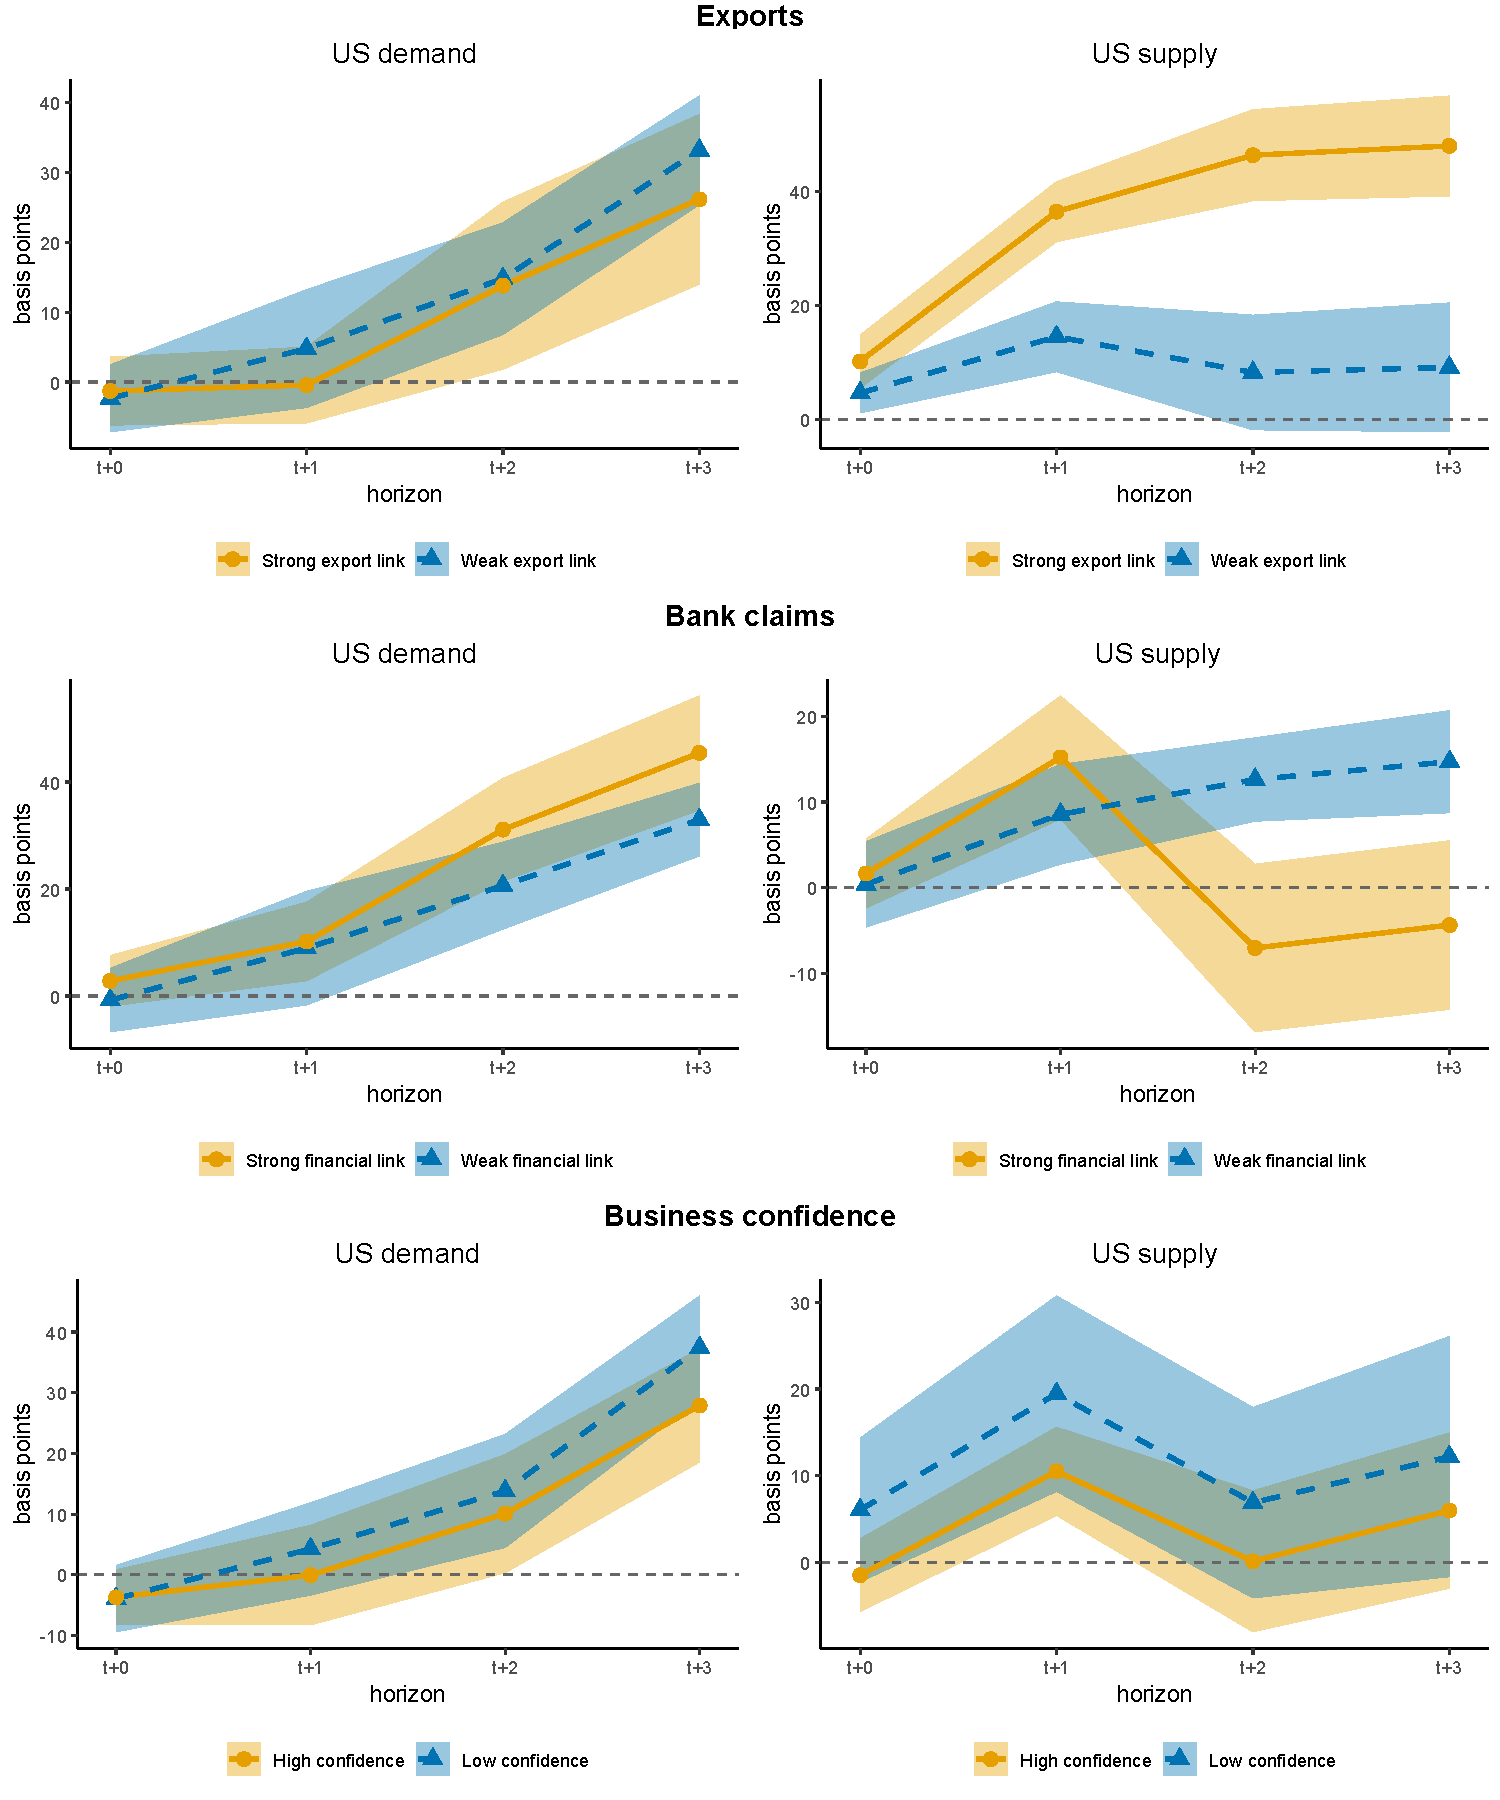
\includegraphics[width=0.80\textwidth]{Figures/State_Dependent_IRFs_with_CI_Final2.pdf}
    \centering \caption*{Note: levels are data-driven, i) exports (weak: up to 50th percentile; strong: 90th percentile), ii) bank claims (weak: 25th percentile, strong: 75th percentile), iii) business confidence (low: 25th percentile, high: 75th percentile). Shaded areas represent 68\% Driscoll-Kraay confidence bands.}
\end{figure}

% Channels - Oleg: this is generated using subsample_channels.r script
\begin{figure}[H]
    \centering    
    \caption{Cumulative impulse responses to demand and supply shocks: transmission channels of US shocks across subsamples.}    
    \label{fig:demand_supply_channels}
    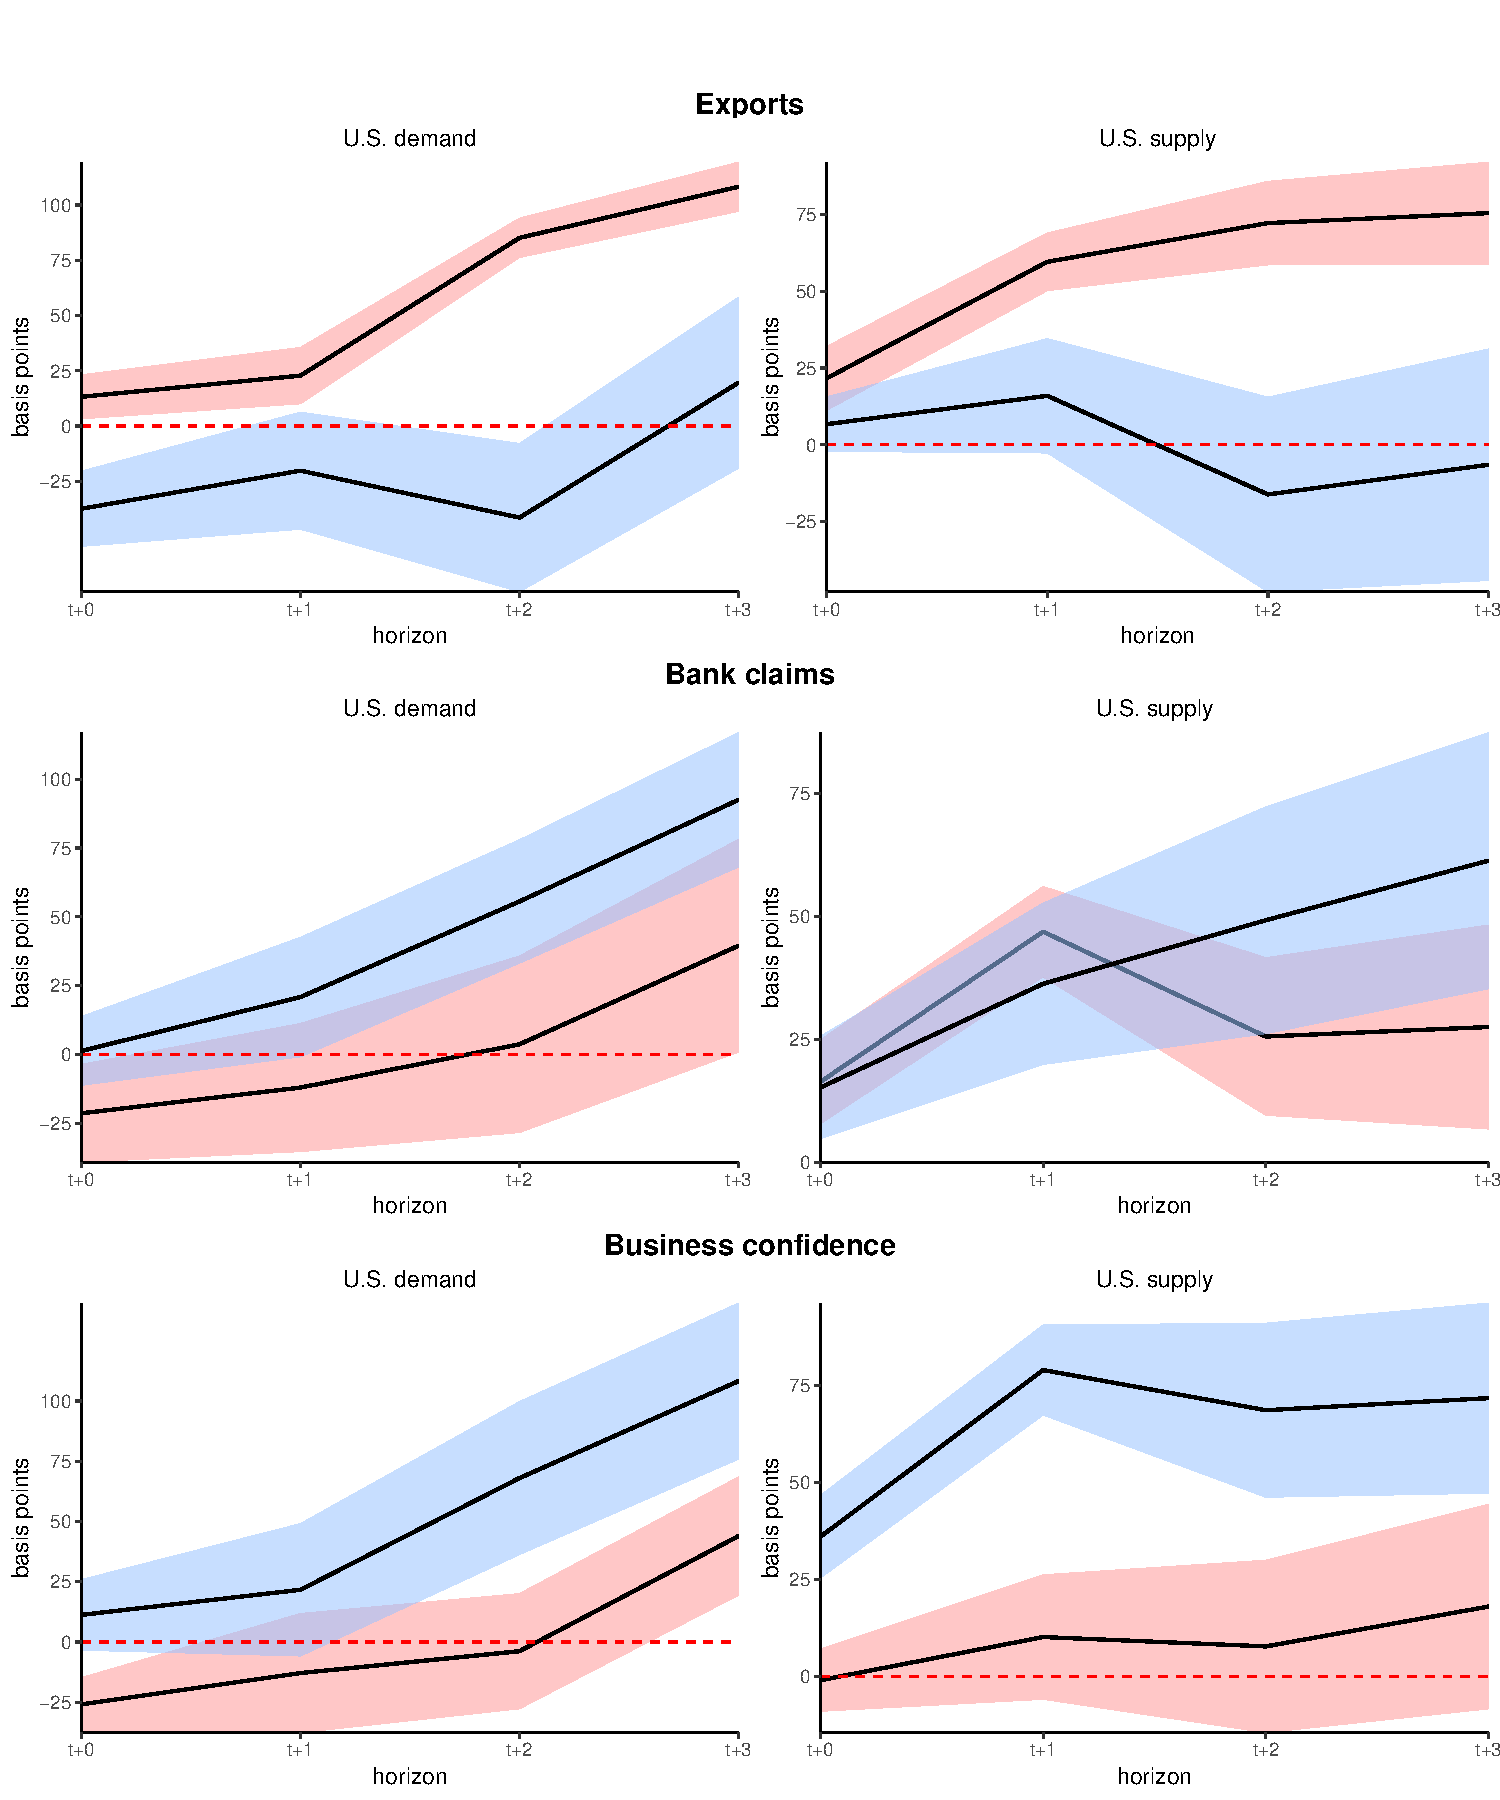
\includegraphics[width=0.75\textwidth]{Figures/high_low_LP_channels_US.pdf}
   \centering \caption*{Note: red response represents \say{high} subsample, blue response represents \say{low} subsample. Sample splitting is done using pooled country-level medians of each measure. Sample composition: i) exports (high exposure: Canada, Germany, Italy, Mexico, Sweden; low exposure: Denmark, France, Norway, Spain), ii) bank claims (high exposure: Canada, Denmark, France, Germany, Mexico; low exposure: Italy, Norway, Spain, Sweden), iii) business confidence (high confidence: France, Italy, Mexico, Norway, Spain; low confidence: Canada, Denmark, Germany, Sweden). Shaded areas represent 68\% Driscoll-Kraay confidence bands.}
\end{figure}

% Gender 
%\begin{figure}[H]
%    \centering    
%    \caption{Cumulative impulse responses to demand and supply shocks: Gini %(by gender), baseline.}    
%    \label{fig:demand_supply_gender_base}
%    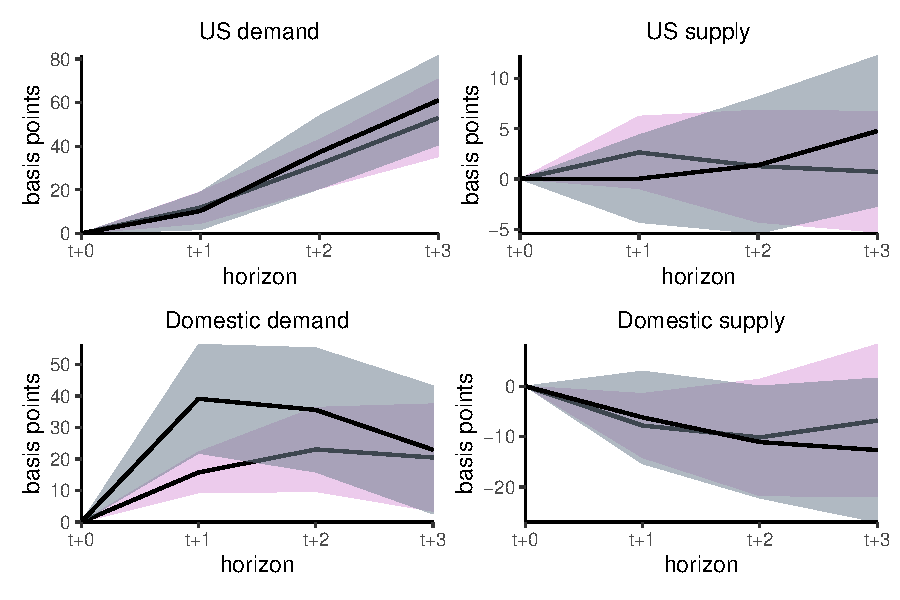
\includegraphics[width=0.85\textwidth]{Figures/baseline_gender_LP_extended.pdf}
%    \centering \caption*{Note: grey response represents men, pink response represents women, shaded areas are 68\% Driscoll-Kraay confidence bands. }
%\end{figure}

%-----------------------------------------------------------------------------
% To be revised
\section{Concluding remarks}
% Findings
In summary, we show that US supply and demand shocks increase income dispersion abroad. While demand shocks have widespread impacts, supply shocks appear more selective, with larger effects concentrated in trade-linked economies. The financial channel does not appear particularly relevant on our estimations. Domestic demand shocks tend to be weaker and more transient. Unlike US supply shocks, domestic shocks reduce inequality.

A more countries join the GRID project, it would become feasible to study the external validity of these findings. Another extension is to consider alternative measures of unanticipated shocks, which can be derived for all countries. 

%-----------------------------------------------------------------------------
% Bibliography
\newpage
\printbibliography
%-----------------------------------------------------------------------------
% Appendix
\pagebreak
\section*{Appendix}
\renewcommand{\thetable}{A\arabic{table}}
\renewcommand{\thefigure}{B\arabic{figure}}
\setcounter{figure}{0}
\setcounter{table}{0}
\subsection*{Part A: Data} \label{appendix:a}
%-----------------------------------------------------------------------------
% Table A1: Time series description
\begin{table}[H]
\captionsetup{justification=raggedright, singlelinecheck=false}
    \centering
    \caption{Real output and unemployment series used for estimation of domestic supply and demand shocks using long-run restrictions.}
    \begin{tabular}{lcc}
    \toprule
       Country & Scope & Source  \\
    \midrule
       Canada (CAN) & 1990:Q2-2019:Q3 & OECD \\
       Denmark (DKK) & 1990:Q2-2019:Q3 & OECD \\
       France (FRA) & 1990:Q2-2019:Q3 & OECD \\
       Germany (DEU) & 1991:Q1-2019:Q3 & OECD \\
       Italy (ITA) & 1990:Q2-2019:Q3 & OECD \\
       Mexico (MEX) & 1990:Q2-2019:Q3 & OECD \\
       Norway (NOR) & 1990:Q2-2019:Q3 & OECD \\
       Spain (ESP) & 1990:Q2-2019:Q3 & OECD \\
       Sweden (SWE) & 1990:Q2-2019:Q3 & OECD \\
       United States (USA) & 1990:Q2-2019:Q3 & FRED \\
    \bottomrule 
    \end{tabular}
    \begin{minipage}{\textwidth}
    \vspace{0.1cm}
    \footnotesize Note: own summary, all data are quarterly. For the USA, we used GDPC1 and UNRATE series. For OECD countries, we used quarterly real GDP (expenditure approach, in USD) and the quarterly unemployment rate (seasonally adjusted, working-age population).
    \end{minipage}
    \label{table:a1}
\end{table}

%-----------------------------------------------------------------------------
% Oleg: Tables A2-A3 moved to the main  text

%-----------------------------------------------------------------------------

% Table A4: control variables
\begin{table}[H]
\captionsetup{justification=raggedright,
singlelinecheck=false
}
\centering
\caption{Control variables used in the estimation of local projections.}
\adjustbox{max width=\textwidth}{%
\begin{tabular}{lcc}
\toprule
  \textbf{Variable} & \textbf{Source}  & \textbf{Availability}
\tabularnewline
\midrule
  NBER identified economic recessions in the US & NBER & 1990-2019\\
  De facto component of the KOF Economic Globalization index  & \textcite{Gygli2019} & 1990-2017 \\
  Labor market regulations score (Area 5) & Fraser Institute & 1990,1995,2000-2019\\
  Share of exports to the US & Own estimation based on UNCTAD & 1990-2019, with gaps \\
  Bilateral US bank claims to GDP & Own estimation based on BIS & 1990-2019, with gaps \\
  Business confidence index & OECD & 1990-2019, with gaps
\tabularnewline
\bottomrule
\end{tabular}}
\begin{minipage}[t]{\textwidth}
\vspace{0.1cm}
\footnotesize Note: own summary.\\
\end{minipage}
\label{table:a4}
\end{table}
%-----------------------------------------------------------------------------



% Table A5: panel data coverage (revised variant)
%\begin{table}[H]
%\captionsetup{justification=raggedright, singlelinecheck=false}
%    \centering
%    \caption{Availability of GRID data (baseline sample).}
%    \begin{tabular}{l c c c c}
%    \toprule
%       Country & Scope & mean Gini & mean Gini (M) & mean Gini (F) \\
%    \midrule
%       Canada   & 1990-2019  & 0.41 (0.01) & 0.40 (0.02) & 0.38 (0.01) \\ 
%       Denmark  & 1990-2016  & 0.28 (0.01) & 0.27 (0.02) & 0.25 (0.01) \\ 
%       France   & 1991-2016  & 0.34 (0.00) & 0.34 (0.01) & 0.32 (0.00) \\ 
%       Germany  & 2001-2016  & 0.40 (0.01) & 0.36 (0.02) & 0.39 (0.01) \\ 
%       Italy    & 1990-2016  & 0.36 (0.02) & 0.34 (0.02) & 0.35 (0.02) \\ 
%       Mexico   & 2005-2019  & 0.56 (0.00) & 0.57 (0.00) & 0.54 (0.01) \\ 
%       Norway   & 1993-2017  & 0.33 (0.01) & 0.31 (0.02) & 0.32 (0.01) \\ 
%       Spain    & 2005-2018  & 0.40 (0.01) & 0.39 (0.02) & 0.39 (0.01) \\ 
%       Sweden   & 1990-2016  & 0.30 (0.01) & 0.28 (0.01) & 0.28 (0.01) \\ 
%    \midrule
%       \multicolumn{1}{l}{N} & \multicolumn{4}{l}{217} \\
%    \bottomrule
%    \end{tabular}
%    
%    \vspace{0.2cm}
%    \raggedright\footnotesize Note: standard deviations in parenthesis, all data are annual.
%    \label{table:a5}
%\end{table}
%-----------------------------------------------------------------------------

% Table A6: within country shock correlations

% \begin{table}[H]
% \captionsetup{justification=raggedright,
% singlelinecheck=false
% }
%     \centering
%     \caption{Correlation coefficients (within country) between supply and demand shocks.}
%     \begin{tabular}{lc}
%     \toprule
%     Country & Correlation \\
%     \midrule
%   CAN & -0.00 \\ 
%   DKK & 0.00 \\ 
%   DEU & 0.00 \\ 
%   ESP & -0.00 \\ 
%   FRA & -0.00 \\ 
%   ITA & 0.00 \\ 
%   MEX & -0.00 \\ 
%   NOR & 0.00 \\ 
%   SWE & -0.00 \\ 
%   USA & -0.00 \\ 
%     \bottomrule
%     \end{tabular}
    
%     \begin{minipage}{9.8cm}
%     \vspace{0.1cm}
%     \footnotesize Note: own summary, shocks are obtained using long-run restrictions. The period under analysis is 1990:Q2-2019:Q3 for all countries except Germany (1991:Q2-2019:Q3).\\  
%     \end{minipage}
%     \label{table:a6}
% \end{table}

% Table A6 - shock statistics

%\begin{table}[ht]
%\centering
%\caption{Summary statistics for demand and supply shocks.}
%\label{table:a6}
%\begin{tabular}{lrrrr}
%  \toprule
%  \multicolumn{5}{c}{\textbf{Before standardization}} \\
%  \midrule
%Statistic & US demand & US supply & Domestic demand & Domestic supply \\
%\midrule
%St. dev. & 0.49 & 0.66 & 0.56 & 0.55 \\
%Mean     & 0.00 & -0.06 & 0.02 & 0.02 \\
%Max      & 0.83 & 0.79 & 4.03 & 3.43 \\
%Min      & -0.75 & -2.36 & -2.01 & -1.73 \\
%\midrule
%\multicolumn{5}{c}{\textbf{After standardization}} \\
%\midrule
%Statistic & US demand & US supply & Domestic demand & Domestic supply \\
%\midrule
%St. dev. & 1.00 & 1.00 & 1.00 & 1.00 \\
%Mean     & 0.00 & 0.00 & 0.00 & 0.00 \\
%Max      & 1.70 & 1.29 & 7.16 & 6.19 \\
%Min      & -1.54 & -3.48 & -3.62 & -3.17 \\
%\bottomrule
%\end{tabular}
%\begin{minipage}{\textwidth}
%\vspace{0.1cm}
%\footnotesize Note: own calculations, all data are annual.
%\end{minipage}
%\end{table}

%-----------------------------------------------------------------------------
% Appendix B for empirical output
\pagebreak
\subsection*{Part B: Local projections and additional results} \label{appendix:b}
\renewcommand{\thetable}{B\arabic{table}}
\setcounter{table}{0}

% 90-10 difference
\begin{figure}[H]
    \centering
    \caption{Cumulative impulse responses to demand and supply shocks: 90-10 percentile difference.}
    \label{fig:9010_demand_supply}
    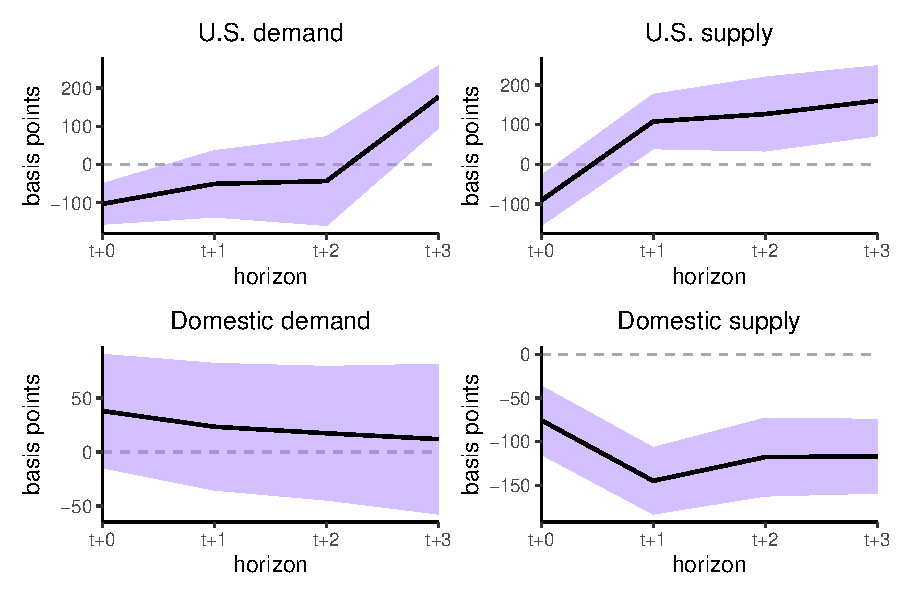
\includegraphics[width=0.75\textwidth]{Figures/p9010_demand_supply_LP.pdf}
    \centering \caption*{Note: shaded areas represent 68\% Driscoll-Kraay confidence bands.}
\end{figure}

% Different lags
\begin{figure}[H]
    \caption{Cumulative responses over longer time horizons.}
    \label{fig:irf_longer}
    \centering
    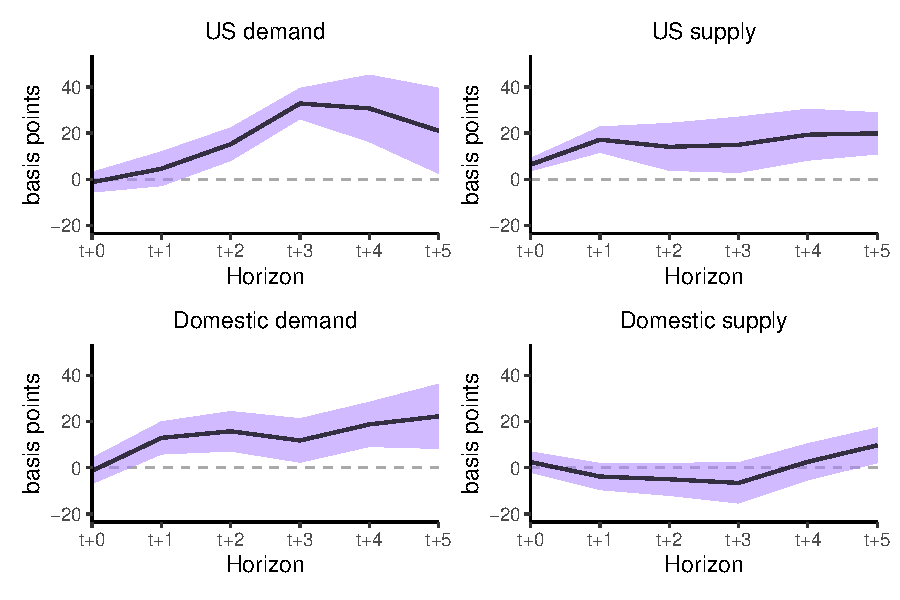
\includegraphics[width=0.75\textwidth]{Figures/baseline_demand_supply_LP5.pdf}
    \caption*{Note: shaded areas represent 68\% Driscoll-Kraay confidence bands.}
\end{figure}

% Robustness
\begin{figure}[H]
    \centering
    \caption{Cumulative impulse responses to demand and supply shocks: Gini, robustness.}
    \label{fig:demand_supply_robust}
    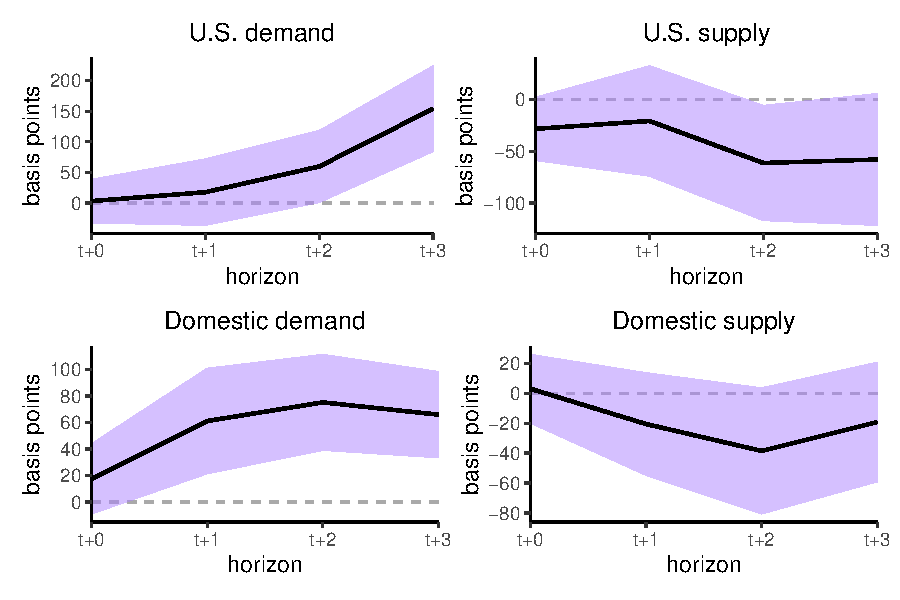
\includegraphics[width=0.75\textwidth]{Figures/robust_demand_supply_LP_extended.pdf}
    \centering \caption*{Note: shaded areas represent 68\% Driscoll-Kraay confidence bands.}
\end{figure}

% Standard deviation with controls
\begin{figure}[H]
    \centering    
    \caption{Cumulative impulse responses to demand and supply shocks: standard deviation, robustness.}  
    \label{fig:std_robust}
    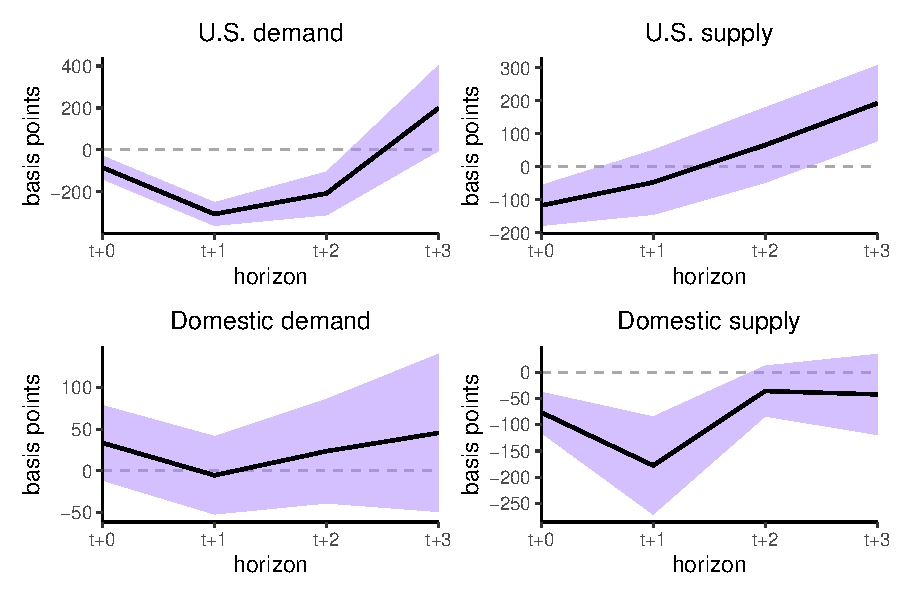
\includegraphics[width=0.75\textwidth]{Figures/std_demand_supply_LP_robust.pdf}
    \centering \caption*{Note: shaded areas represent 68\% Driscoll-Kraay confidence bands.}
\end{figure}

% Kelley with controls
\begin{figure}[H]
    \centering    
    \caption{Cumulative impulse responses to demand and supply shocks: Kelley skewness, robustness.}  
    \label{fig:kelley_robust}
    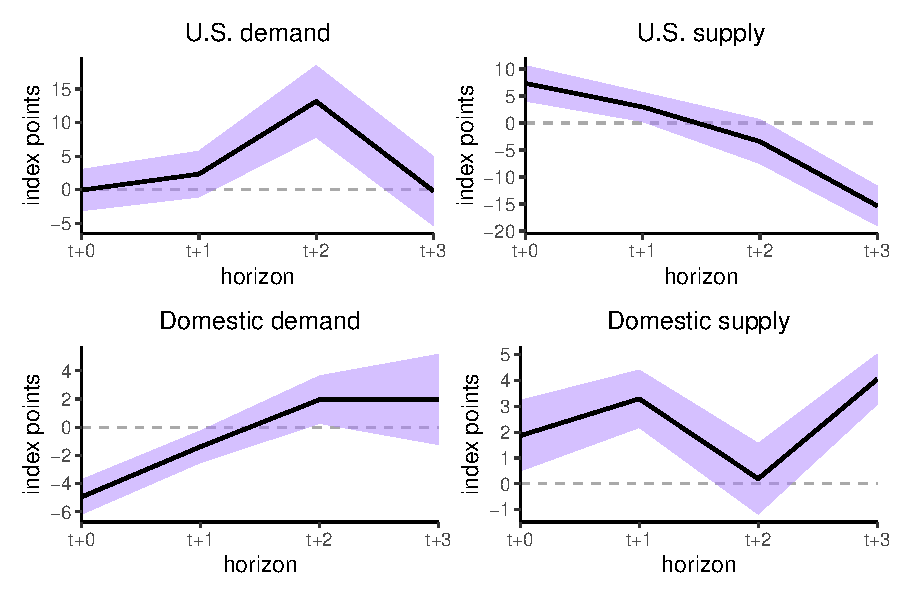
\includegraphics[width=0.75\textwidth]{Figures/kelley_demand_supply_LP_robust.pdf}
    \centering \caption*{Note: shaded areas represent 68\% Driscoll-Kraay confidence bands.}
\end{figure}
%-----------------------------------------------------------------------------
% Gender robust
%\begin{figure}[H]
%    \centering    
%    \caption{Cumulative impulse responses to demand and supply shocks: Gini (by gender), robustness.}    
%    \label{fig:demand_supply_gender_robust}
%    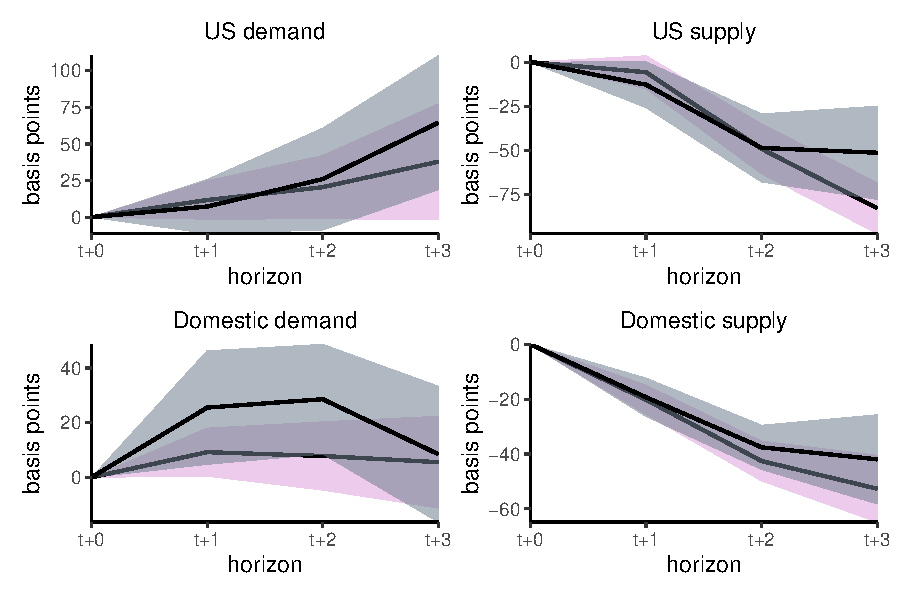
\includegraphics[width=0.80\textwidth]{Figures/robust_gender_LP_extended.pdf}
%    \centering \caption*{Note: grey response represents men, pink response represents women, shaded areas are 68\% Driscoll-Kraay confidence bands.}
%\end{figure}
%-----------------------------------------------------------------------------
% Table - baseline result
\newpage
\begin{table}[!htbp] 
   \centering 
    \caption{Baseline estimation results from local projections, 1990-2019.} 
    \label{tab:a7_baseline_reg_output} 
\resizebox{\textwidth}{!}{%
\begin{tabular}{@{\extracolsep{5pt}}l cccccccc} 
\\[-1.8ex]\hline 
\hline \\[-1.8ex] 
& \multicolumn{8}{c}{\textit{Dependent variable: log (Gini)}} \\ 
\hline \\[-1.8ex]

& \multicolumn{4}{c}{Demand} & \multicolumn{4}{c}{Supply} \\ 
\cmidrule(lr){2-5} \cmidrule(lr){6-9}
& (0) & (1) & (2) & (3) & (0) & (1) & (2) & (3) \\  
\hline \\[-1.8ex] 
%---------------------------------------------------------------------------
% US shocks - verified
%---------------------------------------------------------------------------
\multicolumn{9}{l}{\textit{Model 1:} US shocks} \\[1em]

Shock & $-$0.001 & 0.0001 & 0.001 & 0.003$^{***}$ & 0.001$^{**}$ & 0.002$^{***}$ & 0.001$^{*}$ & 0.002$^{*}$ \\
 & (0.001) & (0.001) & (0.001) & (0.001) & (0.0003) & (0.0005) & (0.001) & (0.001) \\ [0.5em]
 
Shock$_{t-1}$  & 0.001$^{***}$ & 0.002$^{***}$ & 0.003$^{***}$ & 0.002 & 0.001$^{***}$ & 0.001 & 0.002 & 0.002$^{**}$ \\
 & (0.0004) & (0.001) & (0.001) & (0.001) & (0.001) & (0.001) & (0.001) & (0.001) \\ [0.5em]

Shock$_{t-2}$ & 0.001$^{*}$ & 0.001 & 0.001 & 0.001$^{**}$ & 0.0005 & 0.001 & 0.001 & 0.0005 \\
 & (0.001) & (0.001) & (0.001) & (0.001) & (0.001) & (0.001) & (0.001) & (0.001) \\ [0.5em]

$\Delta$ Gini$_{t-1}$ & $-$0.001 & $-$0.0001 & $-$0.001 & $-$0.001 & $-$0.001 & 0.00000 & $-$0.002 & $-$0.001 \\ 
  & (0.001) & (0.002) & (0.002) & (0.002) & (0.001) & (0.002) & (0.002) & (0.002) \\ [0.5em]

$\Delta$ Gini$_{t-2}$  & 0.001 & 0.0004 & 0.001 & $-$0.001 & 0.001 & 0.0004 & 0.001 & $-$0.0002 \\ 
  & (0.001) & (0.001) & (0.002) & (0.002) & (0.001) & (0.001) & (0.002) & (0.002) \\ [1em] 
%---------------------------------------------------------------------------
% Domestic shocks - verified
%---------------------------------------------------------------------------
\multicolumn{9}{l}{\textit{Model 2:} Domestic shocks} \\[1em]

Shock & $-$0.0001 & 0.001$^{*}$ & 0.002$^{*}$ & 0.001 & 0.0002 & $-$0.0002 & $-$0.0002 & $-$0.0002 \\
 & (0.001) & (0.001) & (0.001) & (0.001) & (0.0004) & (0.001) & (0.001) & (0.001) \\ [0.5em]
 
Shock$_{t-1}$  & 0.002$^{**}$ & 0.002$^{**}$ & 0.001$^{*}$ & 0.002$^{**}$ & $-$0.0003 & $-$0.001 & $-$0.001 & $-$0.0001 \\
 & (0.001) & (0.001) & (0.001) & (0.001) & (0.0004) & (0.0004) & (0.001) & (0.001) \\ [0.5em]
 
Shock$_{t-2}$ & 0.0005 & 0.0003 & 0.0004 & 0.001 & $-$0.0001 & $-$0.0001 & 0.0003 & 0.001 \\
& (0.0004) & (0.0004) & (0.0005) & (0.001) & (0.0003) & (0.001) & (0.001) & (0.001) \\ [0.5em]

$\Delta$ Gini$_{t-1}$ & $-$0.001 & 0.00000 & $-$0.001 & $-$0.001 & $-$0.001 & 0.0001 & $-$0.0003 & $-$0.0002 \\ 
  & (0.001) & (0.002) & (0.002) & (0.002) & (0.001) & (0.002) & (0.002) & (0.002) \\ [0.5em]

$\Delta$ Gini$_{t-2}$ & 0.001 & 0.0001 & 0.001 & 0.0004 & 0.001 & 0.0004 & 0.001 & 0.001 \\ 
  & (0.001) & (0.001) & (0.002) & (0.002) & (0.001) & (0.001) & (0.002) & (0.002) \\ [1em]
\\[-1.8ex] \hline \\[-1.8ex] 
N & 177 & 168 & 159 & 150 & 177 & 168 & 159 & 150 \\ 
\hline \\[-1.8ex]
\end{tabular}
}
\begin{minipage}{\textwidth}
    \vspace{0.1cm} 
    \footnotesize  Note: Driscoll-Kraay errors in parenthesis, column headers represent estimation horizons. Model 1 includes country fixed effects and NBER recession dummy. Model 2 includes country and year fixed effects. Significance levels: $^{*}$p$<$0.1, $^{**}$p$<$0.05, $^{***}$p$<$0.01.
\end{minipage}
\end{table}
%-----------------------------------------------------------------------------
\newpage
% Table - restricted and robustness coeff 
\begin{table}[!htbp] 
  \caption{The effect of supply and demand shocks on income inequality, 1990-2019.} 
  \label{table:a8}
  \centering
\resizebox{\textwidth}{!}{
\begin{tabular}{@{\extracolsep{5pt}}l cccc || cccc} 
 \hline \hline
 \\[-1.8ex] 
& \multicolumn{8}{c}{\textit{Dependent variable: log (Gini)}} \\\hline \\[-1.8ex]
& \multicolumn{4}{c}{Demand} & \multicolumn{4}{c}{Supply} \\ 
\cmidrule(lr){2-5} \cmidrule(lr){6-9}
\\[-1.8ex] 
& $\beta_t$ & $\beta_{t+1}$ & $\beta_{t+2}$ & $\beta_{t+3}$ & $\beta_t$ & $\beta_{t+1}$ & $\beta_{t+2}$ & $\beta_{t+3}$ \\ \hline
\\[-0.5em] 

% US shocks
\multicolumn{7}{l}{\textit{Panel 1}: US shocks} \\

(a) Baseline & $-$0.001 & 0.0001 & 0.001 & 0.003$^{***}$  &0.001$^{**}$ & 0.002$^{***}$ & 0.001$^{*}$ & 0.002$^{*}$ \\
& (0.001) & (0.001) & (0.001) & (0.001) & (0.0003) & (0.0005) & (0.001) & (0.001) \\
N & 177 & 168 & 159 & 150 & 177 & 168 & 159 & 150 \\ [1em]

% revised with business confidence 
(b) Restricted sample &  0.001 & 0.001 & 0.002 & 0.006$^{***}$ & 0.001 & 0.002 & $-$0.0001 & $-$0.001 \\
& (0.001) & (0.002) & (0.001) & (0.002) & (0.001) & (0.001) & (0.001) & (0.001) \\
N & 118 & 109 & 100 & 91 & 118 & 109 & 100 & 91 \\ [1em]

% revised with business confidence 
(c) All controls  & 0.0002 & 0.001 & 0.003 & 0.007$^{**}$ & $-$0.001 & $-$0.001 & $-$0.003 & $-$0.002 \\
& (0.002) & (0.002) & (0.003) & (0.003) & (0.001) & (0.002) & (0.002) & (0.003) \\
N & 118 & 109 & 100 & 91 & 118 & 109 & 100 & 91 \\ [1em]

% Domestic shocks
\multicolumn{7}{l}{\textit{Panel 2:} Domestic shocks} \\

(a) Baseline  & $-$0.0001 & 0.001$^{*}$ & 0.002$^{*}$ & 0.0002 & 0.0002 & $-$0.0002 & $-$0.0002 & $-$0.0002 \\
 & (0.001) & (0.001) & (0.001) & (0.001) & (0.0004) & (0.001) & (0.001) & (0.001) \\ 
N & 177 & 168 & 159 & 150 & 177 & 168 & 159 & 150 \\ [1em]

% revised with business confidence 
(b) Restricted sample &  0.001 & 0.003$^{**}$ & 0.005$^{***}$ & 0.004$^{**}$ &  0.001 & $-$0.0004 & $-$0.001 & $-$0.001 \\
& (0.001) & (0.002) & (0.002) & (0.002) & (0.001) & (0.001) & (0.002) & (0.002) \\
N & 118 & 109 & 100 & 91 & 118 & 109 & 100 & 91 \\ [1em]

% revised with business confidence 
(c) All controls & 0.001 & 0.003 & 0.003$^{**}$ & 0.003$^{*}$ & 0.0001 & $-$0.001 & $-$0.002 & $-$0.001 \\
& (0.001) & (0.002) & (0.002) & (0.001) & (0.001) & (0.001) & (0.002) & (0.002) \\
N & 118 & 109 & 100 & 91 & 118 & 109 & 100 & 91 \\\hline 

\end{tabular}
}
\begin{minipage}{\textwidth}
    \vspace{0.1cm}
    % revised with business confidence 
    \footnotesize  Note: Driscoll-Kraay errors in parenthesis, columns headers represent estimation horizons. Baseline regressions include additional controls for: growth of Gini (2 lags), shock (2 lags). Restricted sample is computed using baseline regressions, but only including entries, for which we have complete observations for all controls used in the estimation. For all controls, we introduce (2 lags): changes in the KOF index, changes in the labor market regulations, the share of exports to the US, bilateral US bank claims to GDP, and business confidence index. Significance levels: $^{*}$p$<$0.1, $^{**}$p$<$0.05, $^{***}$p$<$0.01.
\end{minipage}
\end{table}


 


%-----------------------------------------------------------------------------
% VAR impluses
\newpage
\begin{figure}[H]
    \caption{Estimated impulse response functions to demand shock.}
    \label{fig:var_impulses_demand}
    \centering
    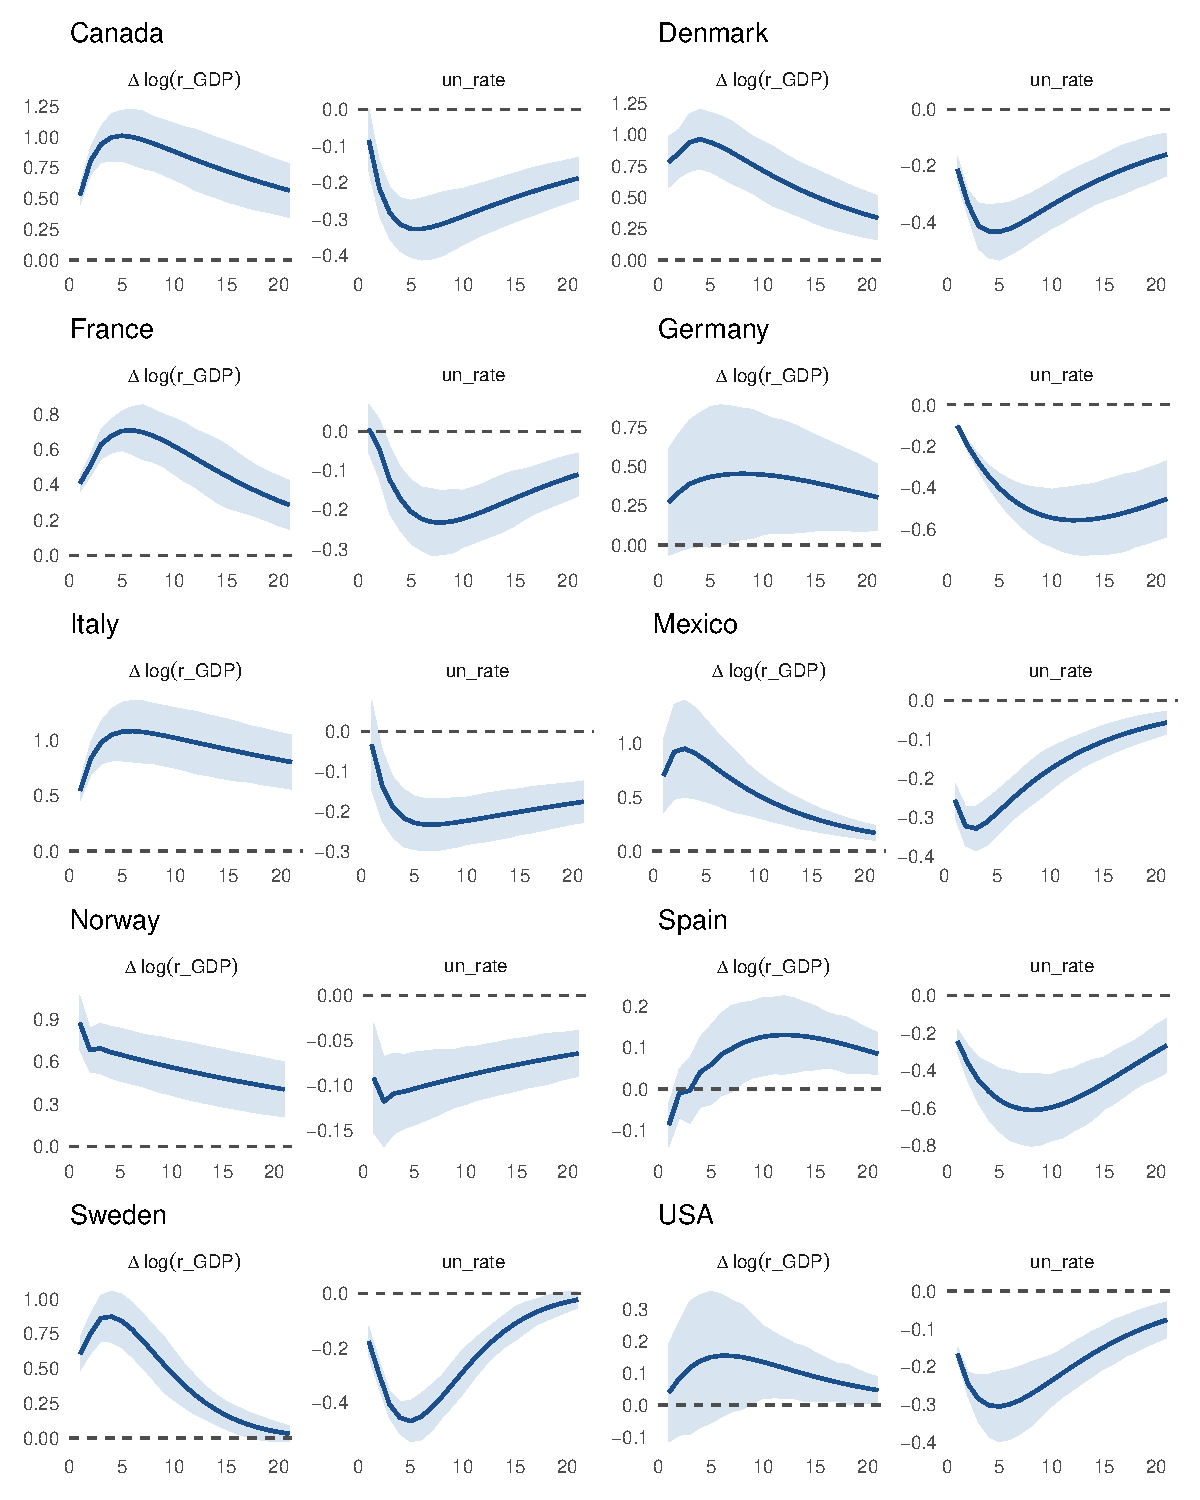
\includegraphics[width=\textwidth, height=0.9\textheight, keepaspectratio]{Figures/all_demand.pdf}
    \caption*{Note: 20 quarters, shaded areas represent 68\% confidence bands. r\_GDP and un\_rate stand for real output growth and unemployment rate.}
\end{figure}

\newpage
\begin{figure}[H]
    \caption{Estimated impulse response functions to supply shock.}
    \label{fig:var_impulses_supply}
    \centering
    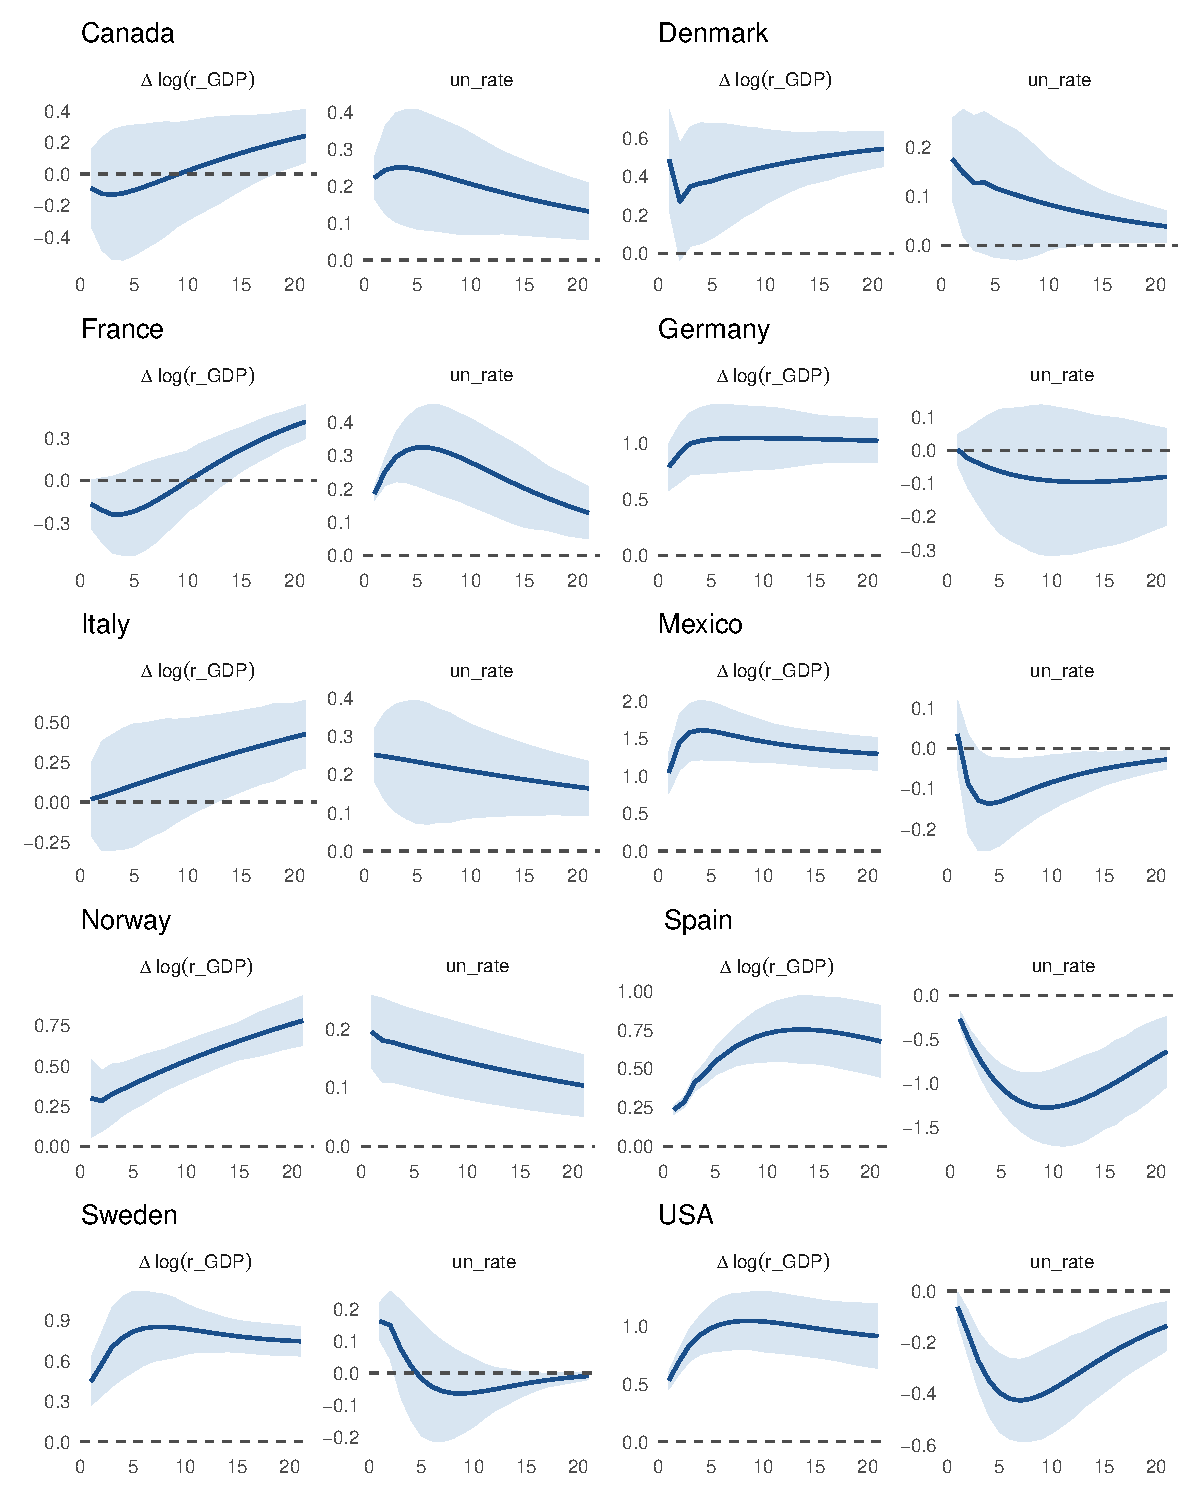
\includegraphics[width=\textwidth, height=0.9\textheight, keepaspectratio]{Figures/all_supply.pdf}
    \caption*{Note: 20 quarters, shaded areas represent 68\% confidence bands. r\_GDP and un\_rate stand for real output growth and unemployment rate.}
\end{figure}
% End
\end{document}